\chapter{Kết quả hiện thực}\label{chap:result}
		Sau quá trình dài thực hiện luận văn, sử dụng những công nghệ và kiên thức được đưa
		ra trong các phần trước, nhóm đã hoàn thành một hệ thống vận chuyển hàng hóa liên tỉnh tương đối hoàn chỉnh.
		
		\section{Chức năng đăng nhập, đăng kí}
			\subsection{Đăng kí}
				\begin{figure}[H]
					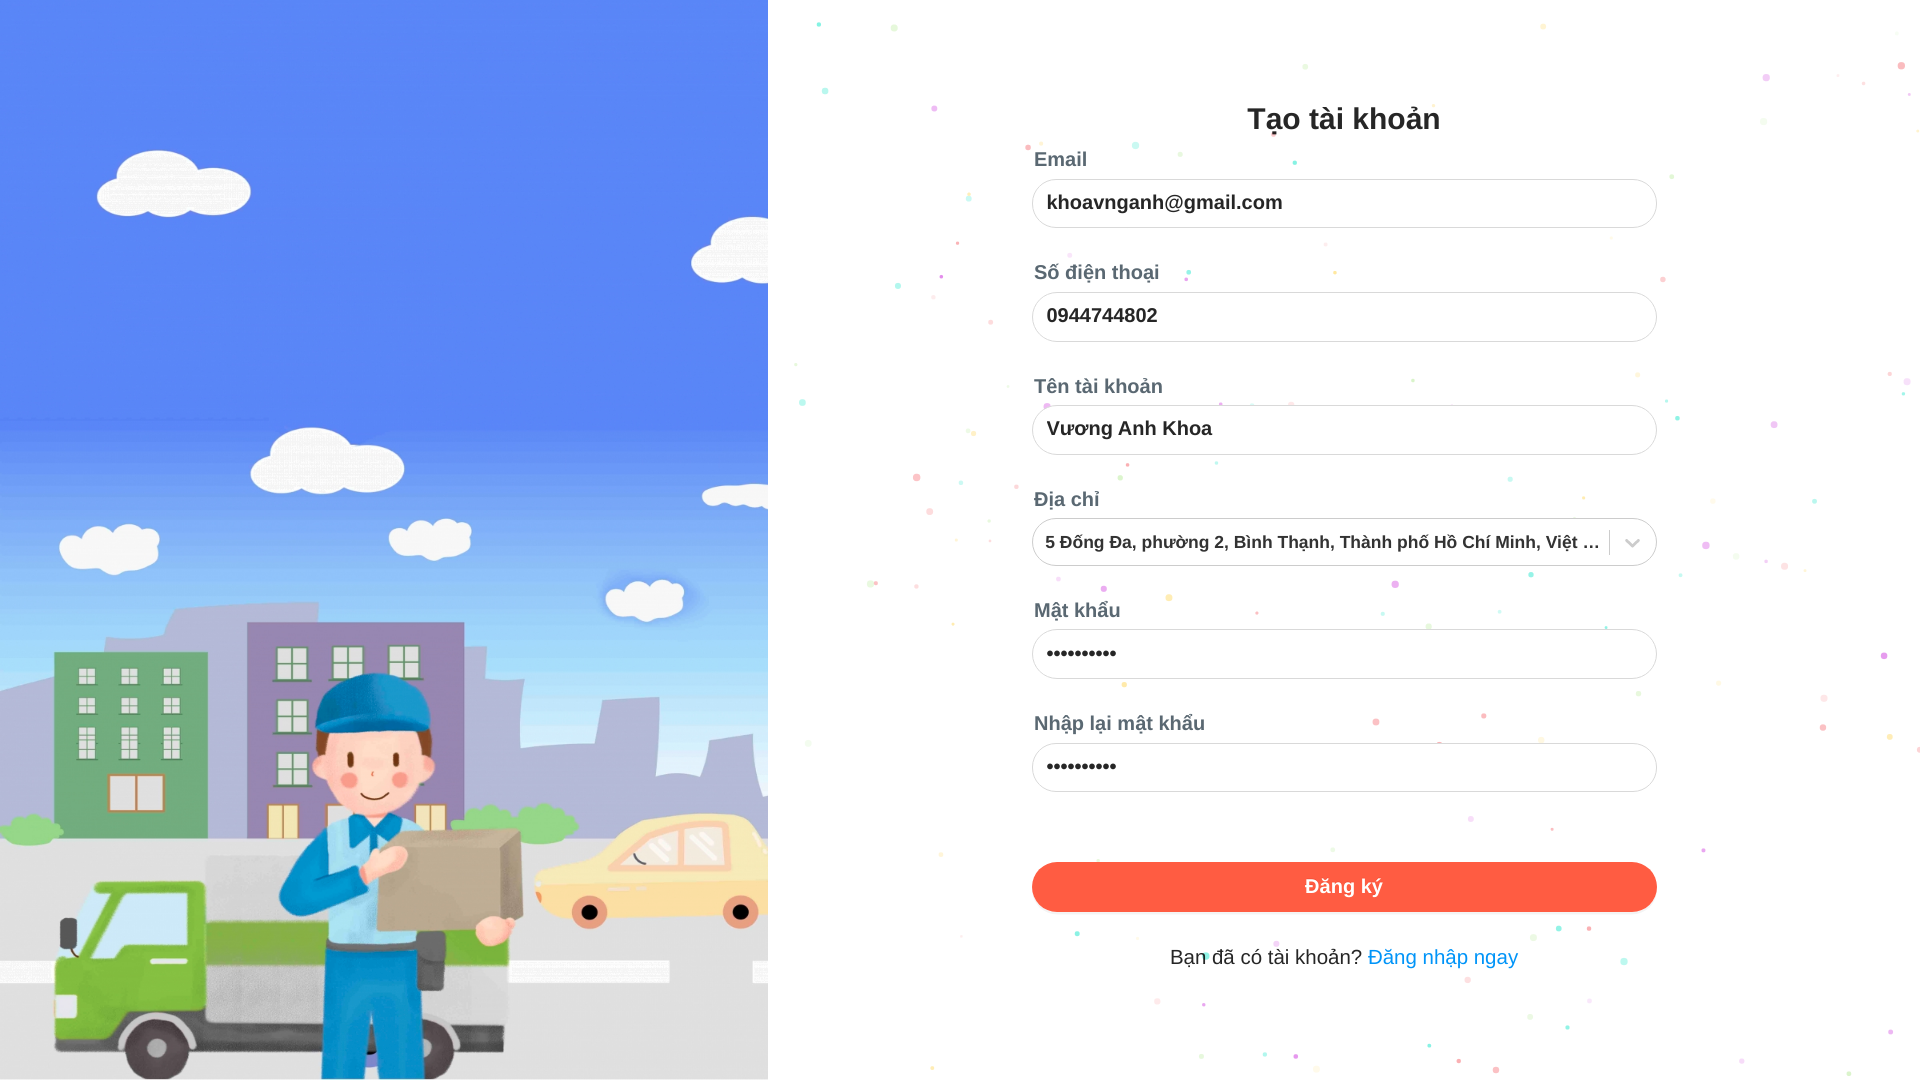
\includegraphics[width=0.8\textwidth]{/Auth/SignUp.png}
					\centering
					\caption{Giao diện đăng kí dành cho người muốn gửi đơn hàng}
				\end{figure}
			
			\subsection{Đăng nhập}
				\begin{figure}[H]
					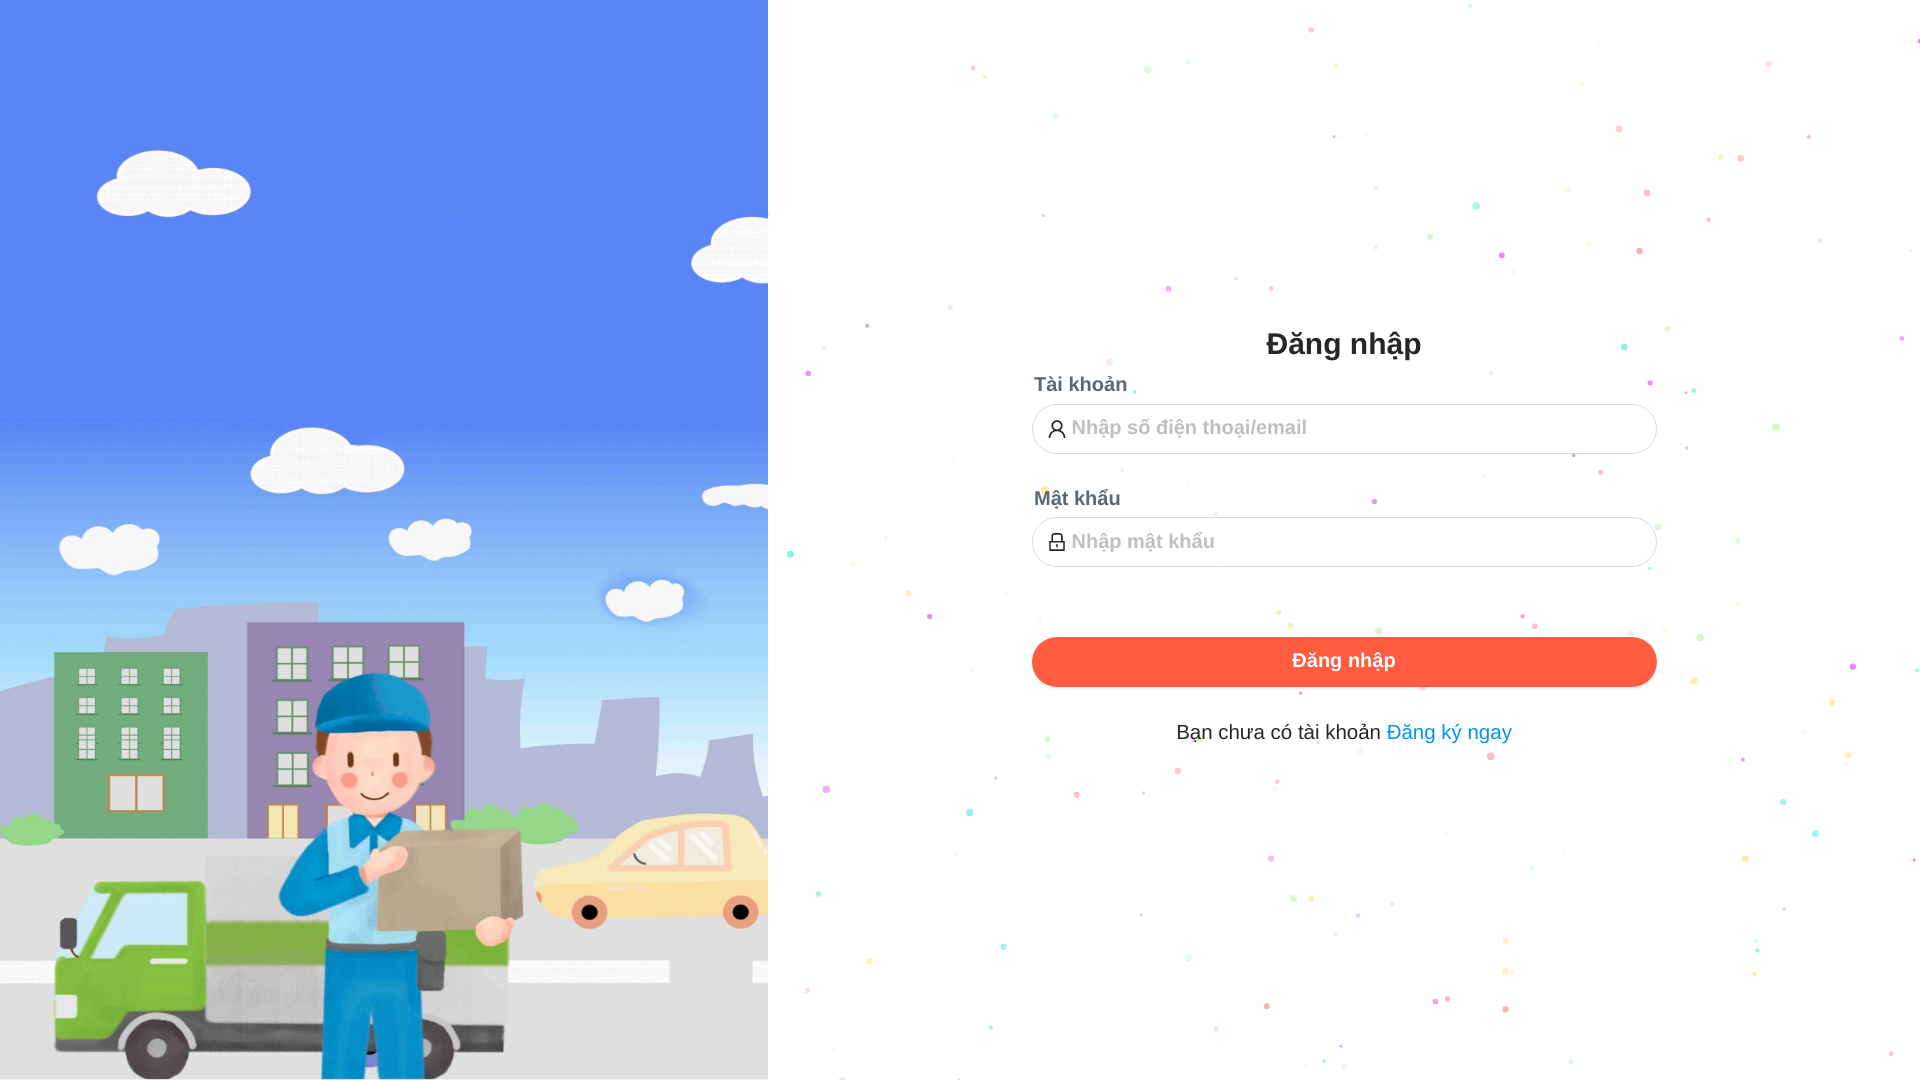
\includegraphics[width=0.8\textwidth]{/Auth/SignIn.png}
					\centering
					\caption{Giao diện đăng nhập dành cho actor của hệ thống}
				\end{figure}
			
			
		\section{Chức năng dành cho người gửi}
			\subsection{Lên yêu cầu gửi hàng}
				\begin{figure}[H]
					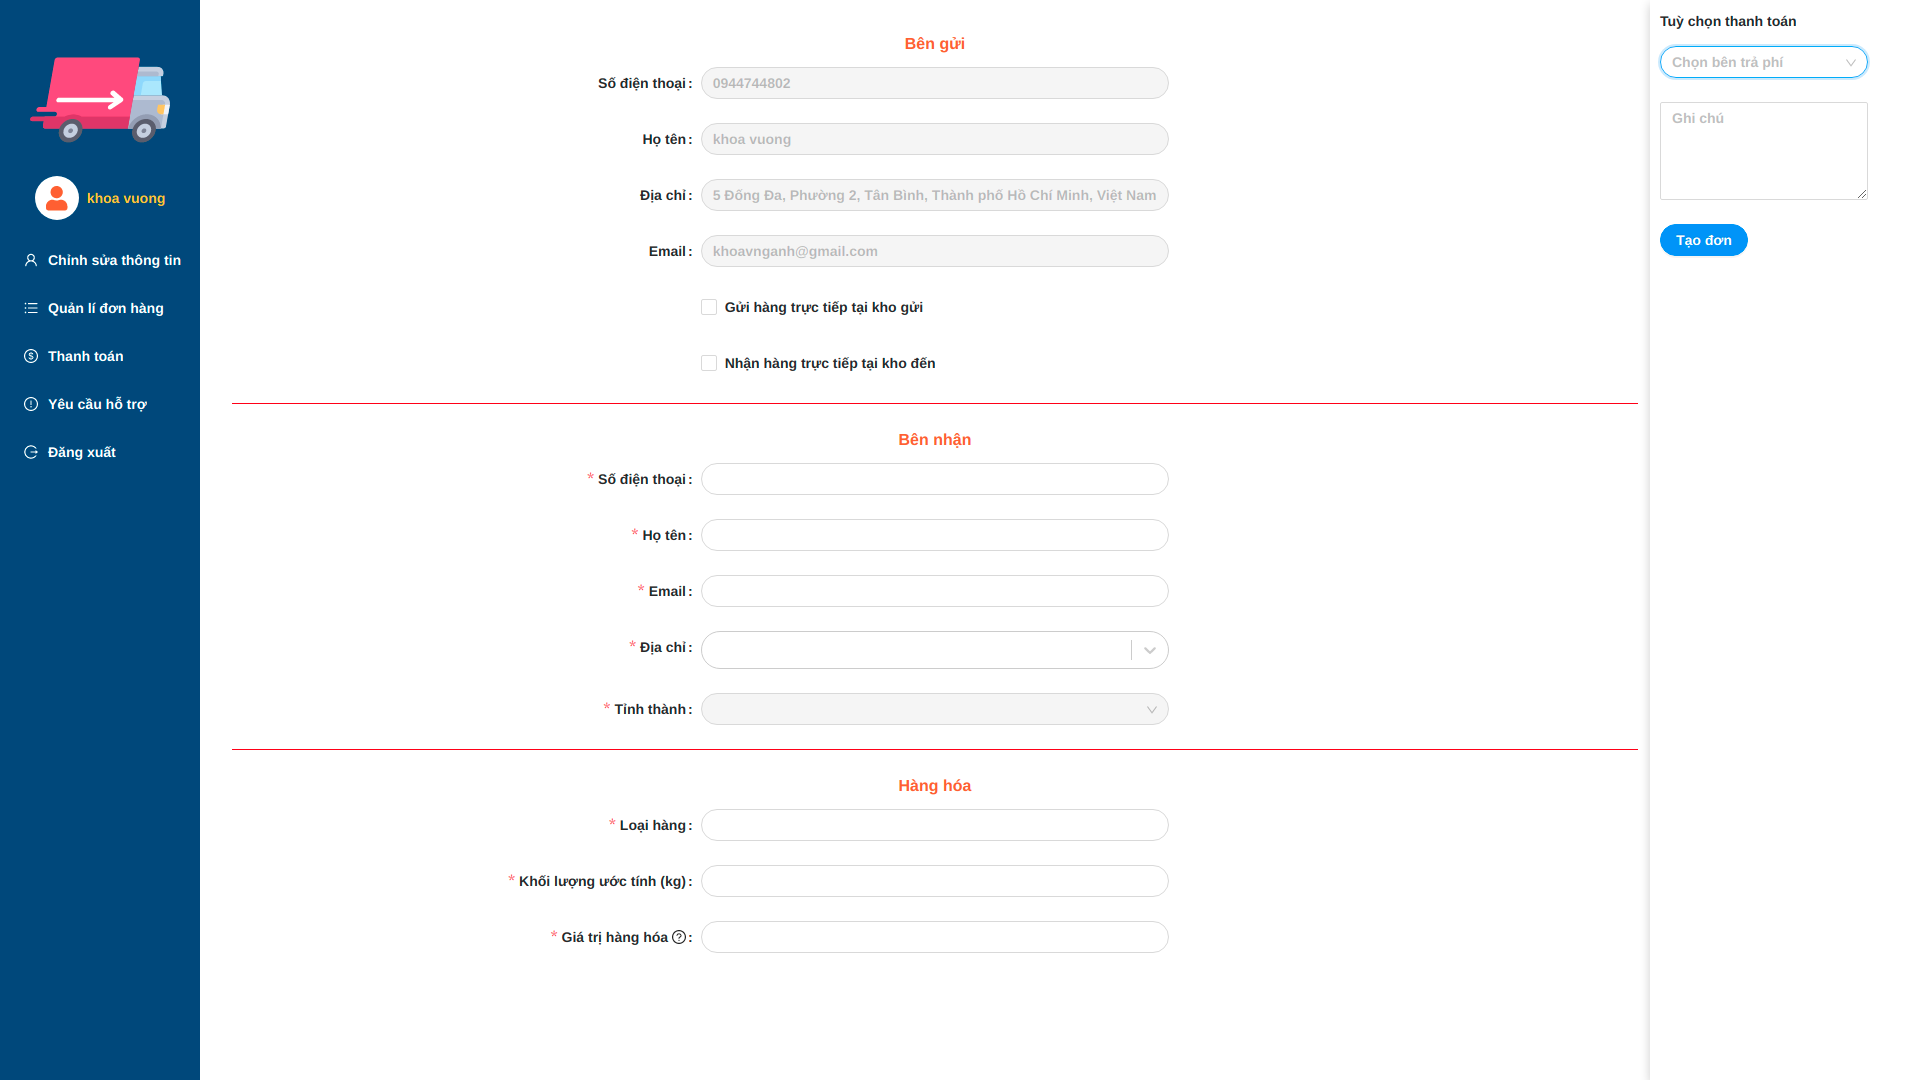
\includegraphics[width=0.8\textwidth]{/sender/create_order.png}
					\centering
					\caption{Giao diện điền thông tin để lên yêu cầu gửi hàng}
				\end{figure}
				
				\begin{figure}[H]
					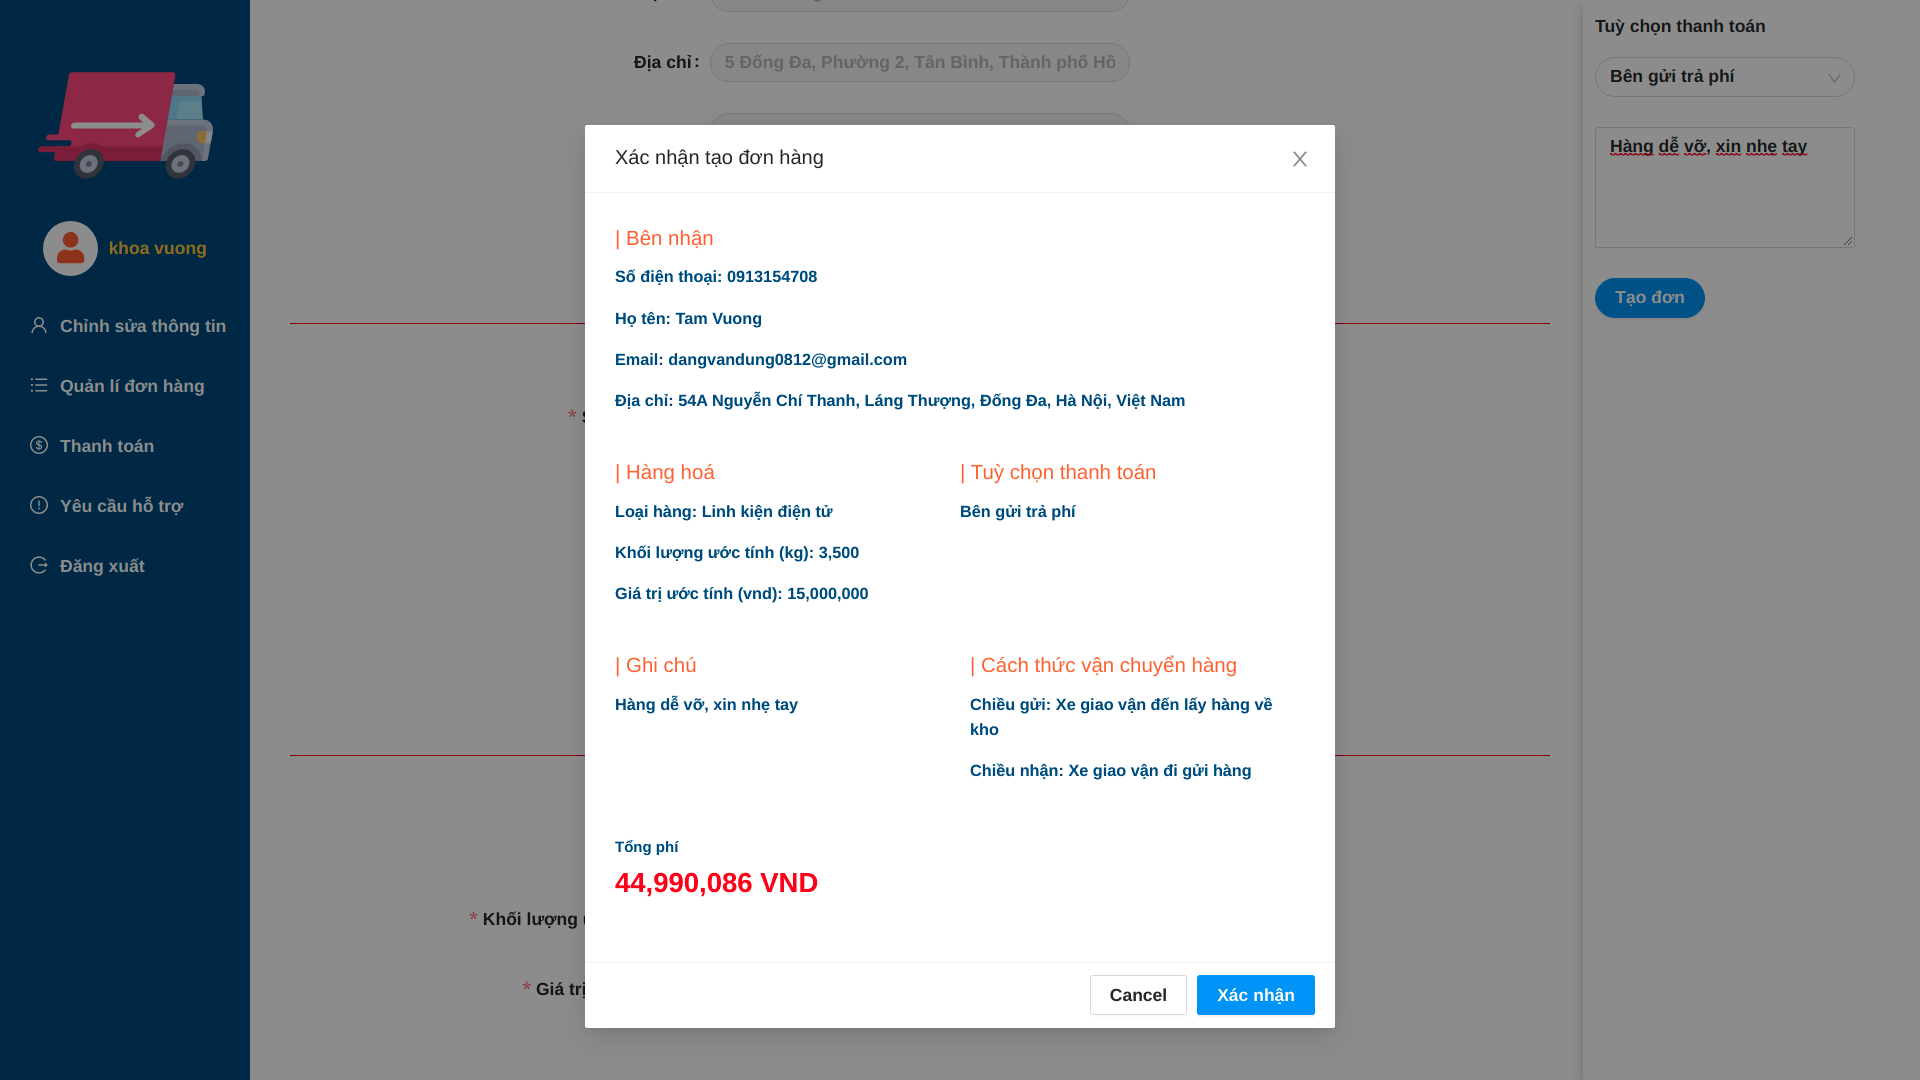
\includegraphics[width=0.8\textwidth]{/sender/create_order_model.png}
					\centering
					\caption{Thông tin xác nhận yêu cầu muốn tạo}
				\end{figure}
				
				Khung nhập địa chỉ hỗ trợ gợi ý địa chỉ nhờ sử dụng Google Place Autocomplete API. Khi ấn nút tạo đơn sẽ có màn hình chờ để phía server trả về phí vận chuyển.
			
		
			\subsection{Xem danh sách yêu cầu đã tạo}
				\begin{figure}[H]
					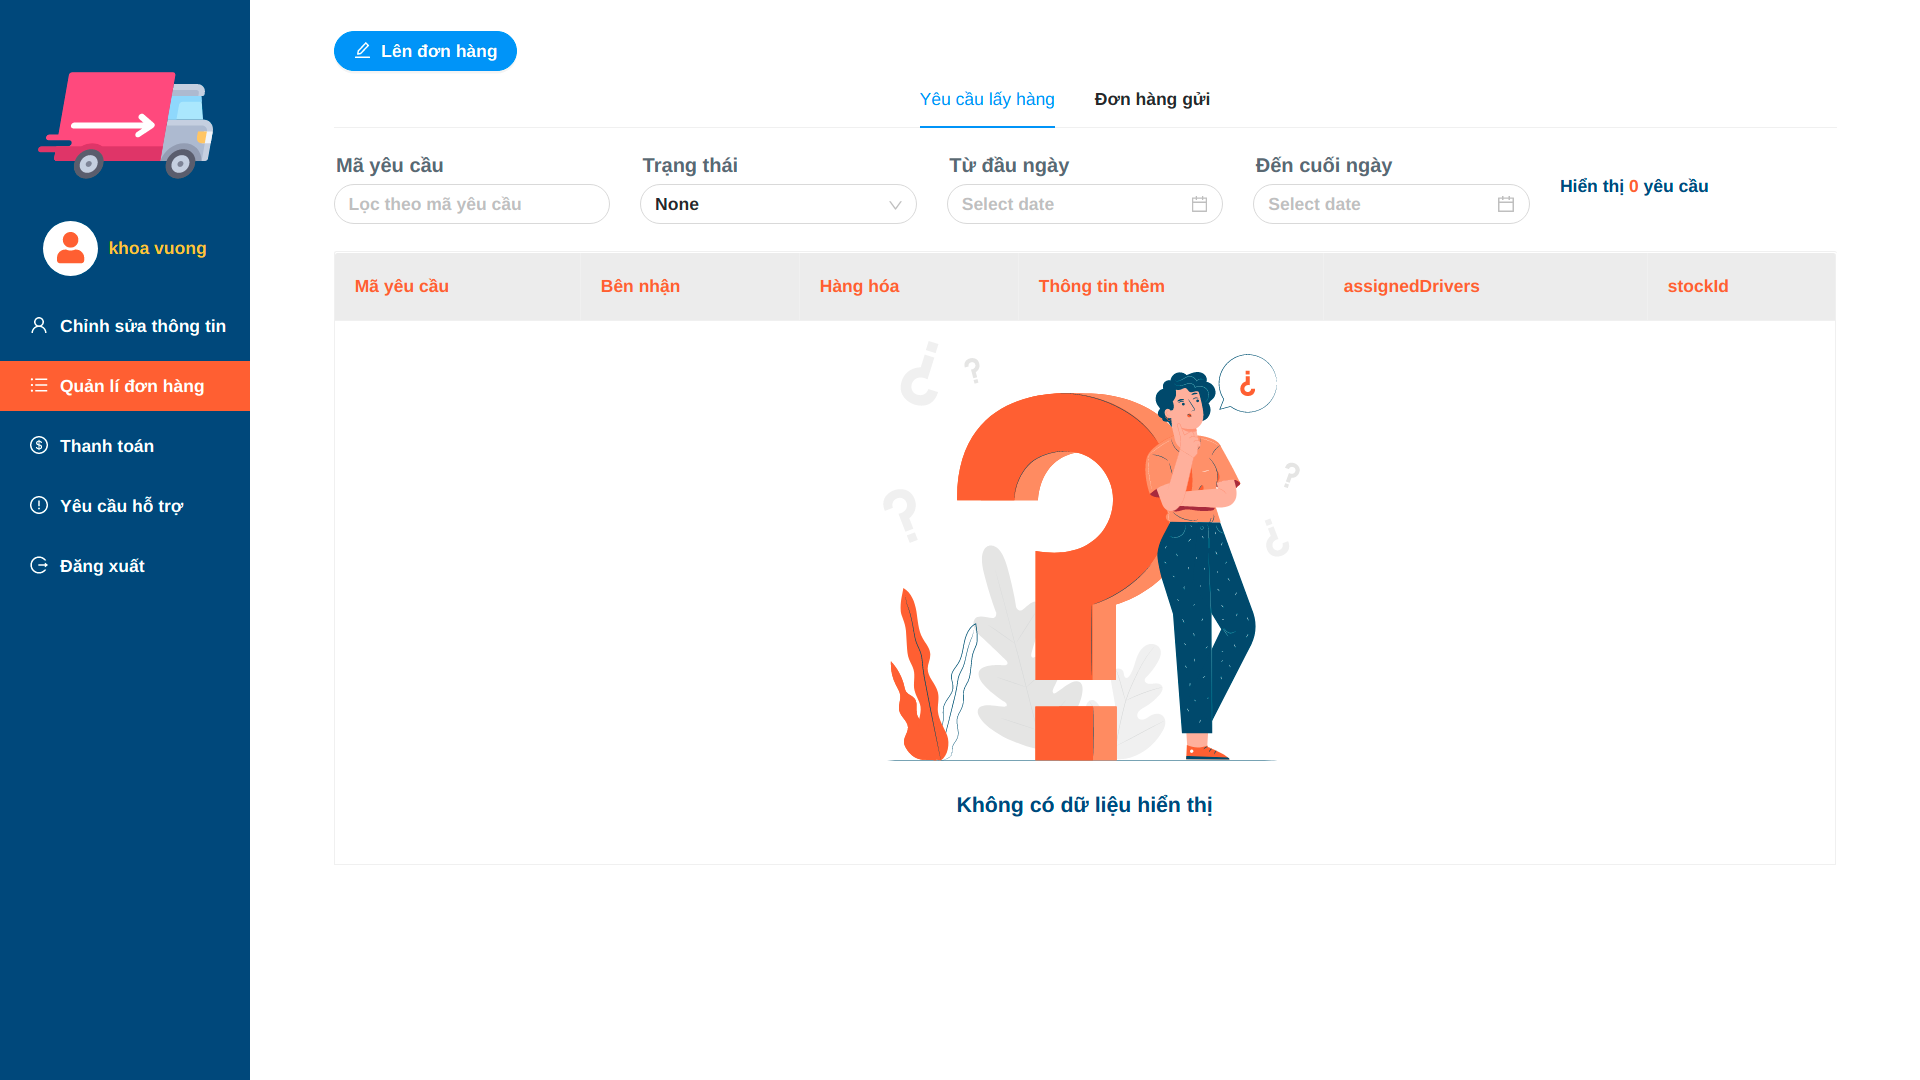
\includegraphics[width=0.8\textwidth]{/sender/request_empty.png}
					\centering
					\caption{Giao diện list yêu cầu của người gửi (Rỗng)}
				\end{figure}
				
				\begin{figure}[H]
					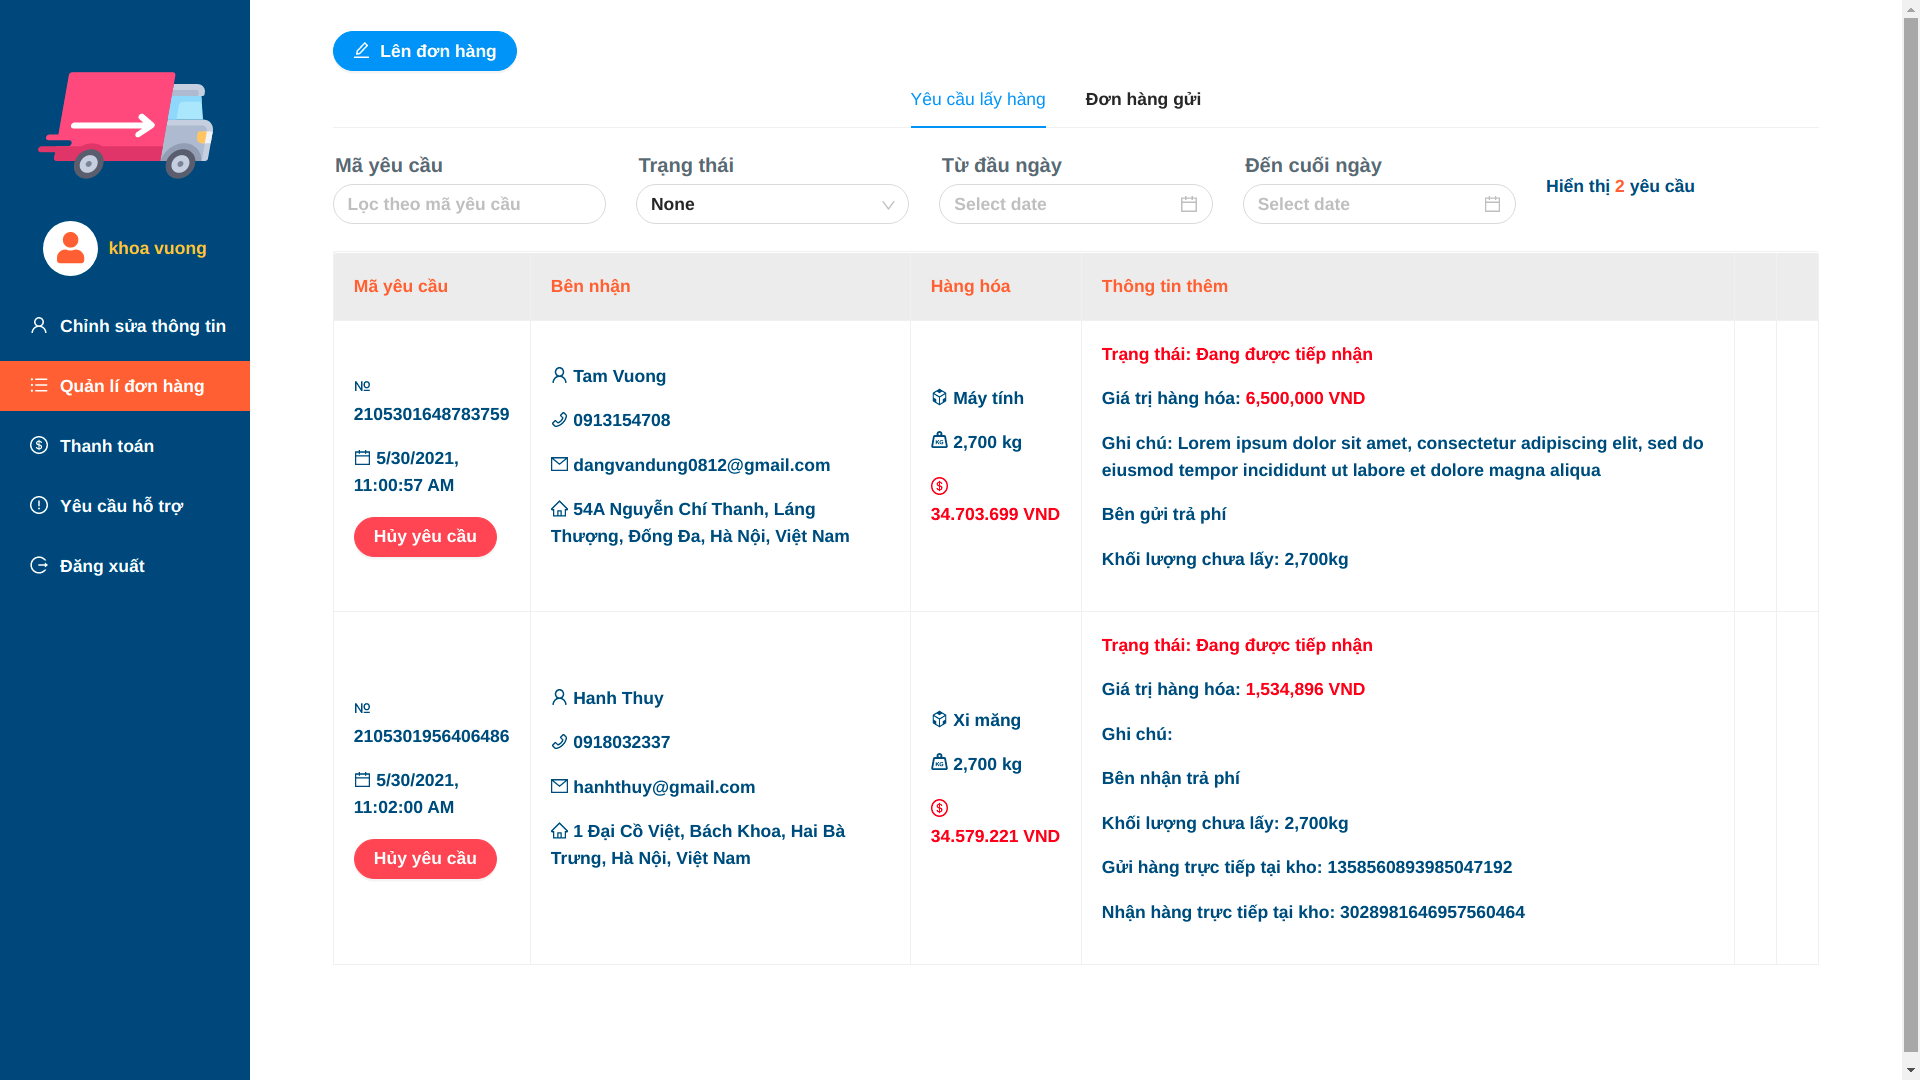
\includegraphics[width=0.8\textwidth]{/sender/request_list.png}
					\centering
					\caption{Giao diện list yêu cầu của người gửi (Có yêu cầu)}
				\end{figure}
		
				Các yêu cầu đã tạo có thể được lọc theo những tiêu chí: Mã yêu cầu, trạng thái (Gồm 4 trạng thái yêu cầu đã nêu trong phần trước), thời gian tạo đơn hàng.
			
			
			\subsection{Xem danh sách các đơn hàng nhỏ được tách từ yêu cầu}
				\begin{figure}[H]
					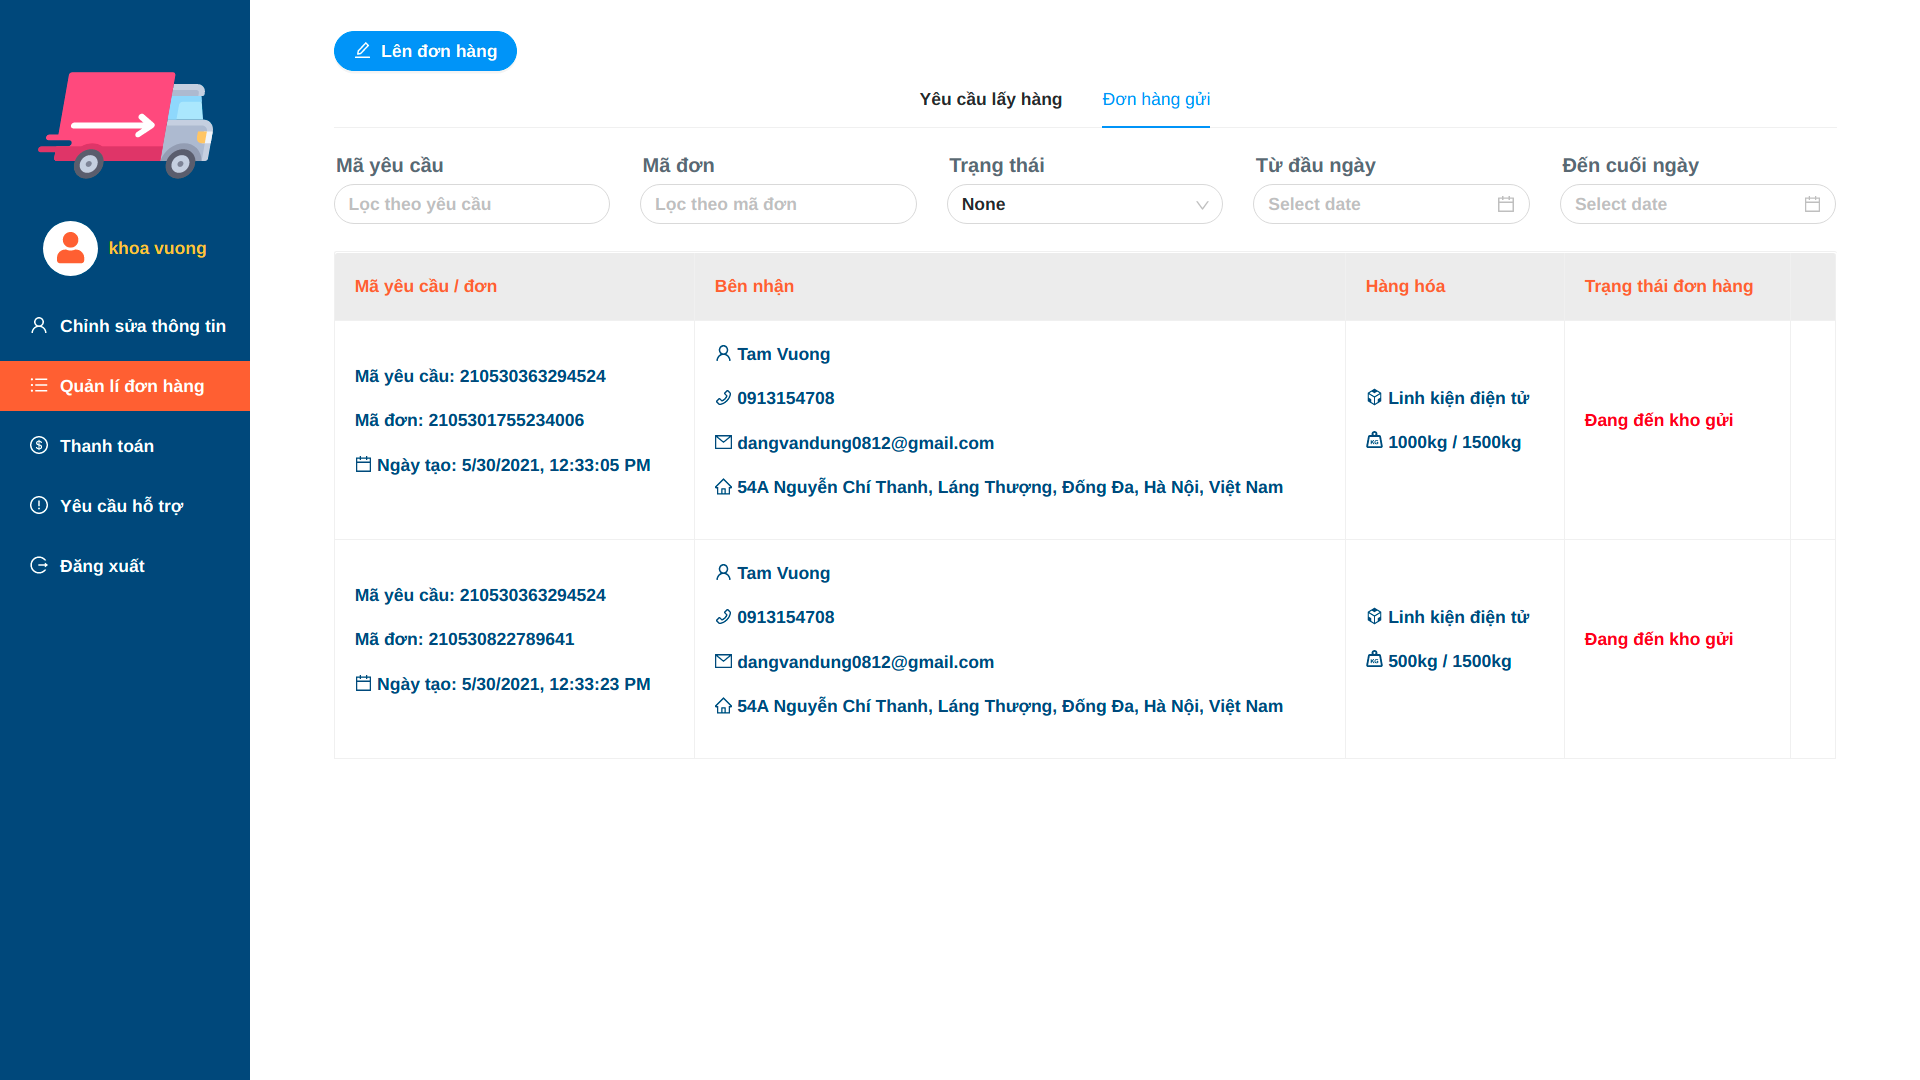
\includegraphics[width=0.8\textwidth]{/sender/sender_suborders.png}
					\centering
					\caption{Giao diện xem danh sách các đơn hàng nhỏ được tách từ yêu cầu}
				\end{figure}
			
			\subsection{Chỉnh sửa thông tin của người gửi}
				\begin{figure}[H]
					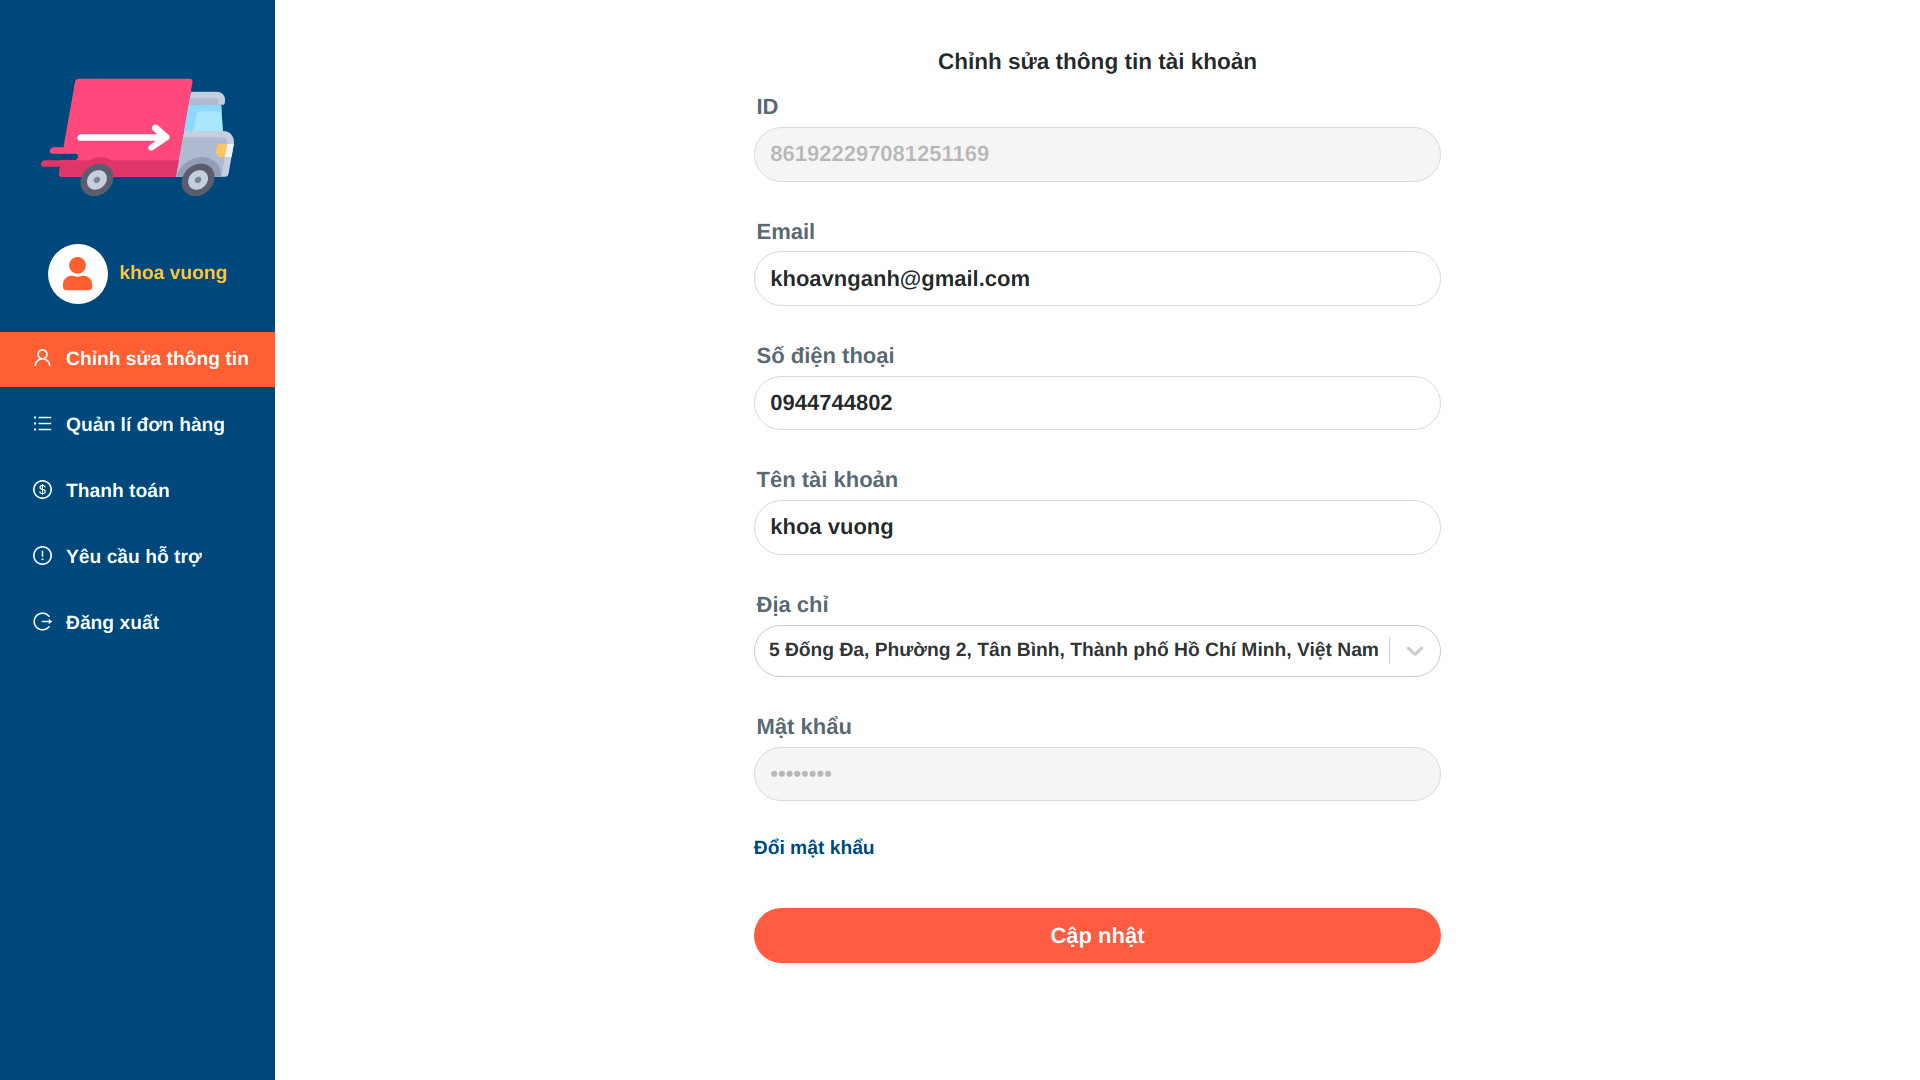
\includegraphics[width=0.8\textwidth]{/sender/sender_info.png}
					\centering
					\caption{Giao diện chỉnh sửa thông tin của người gửi}
				\end{figure}
			
		\section{Chức năng dành cho tài xế}
			\subsection{Tìm những yêu cầu được gán}
				\begin{figure}[H]
					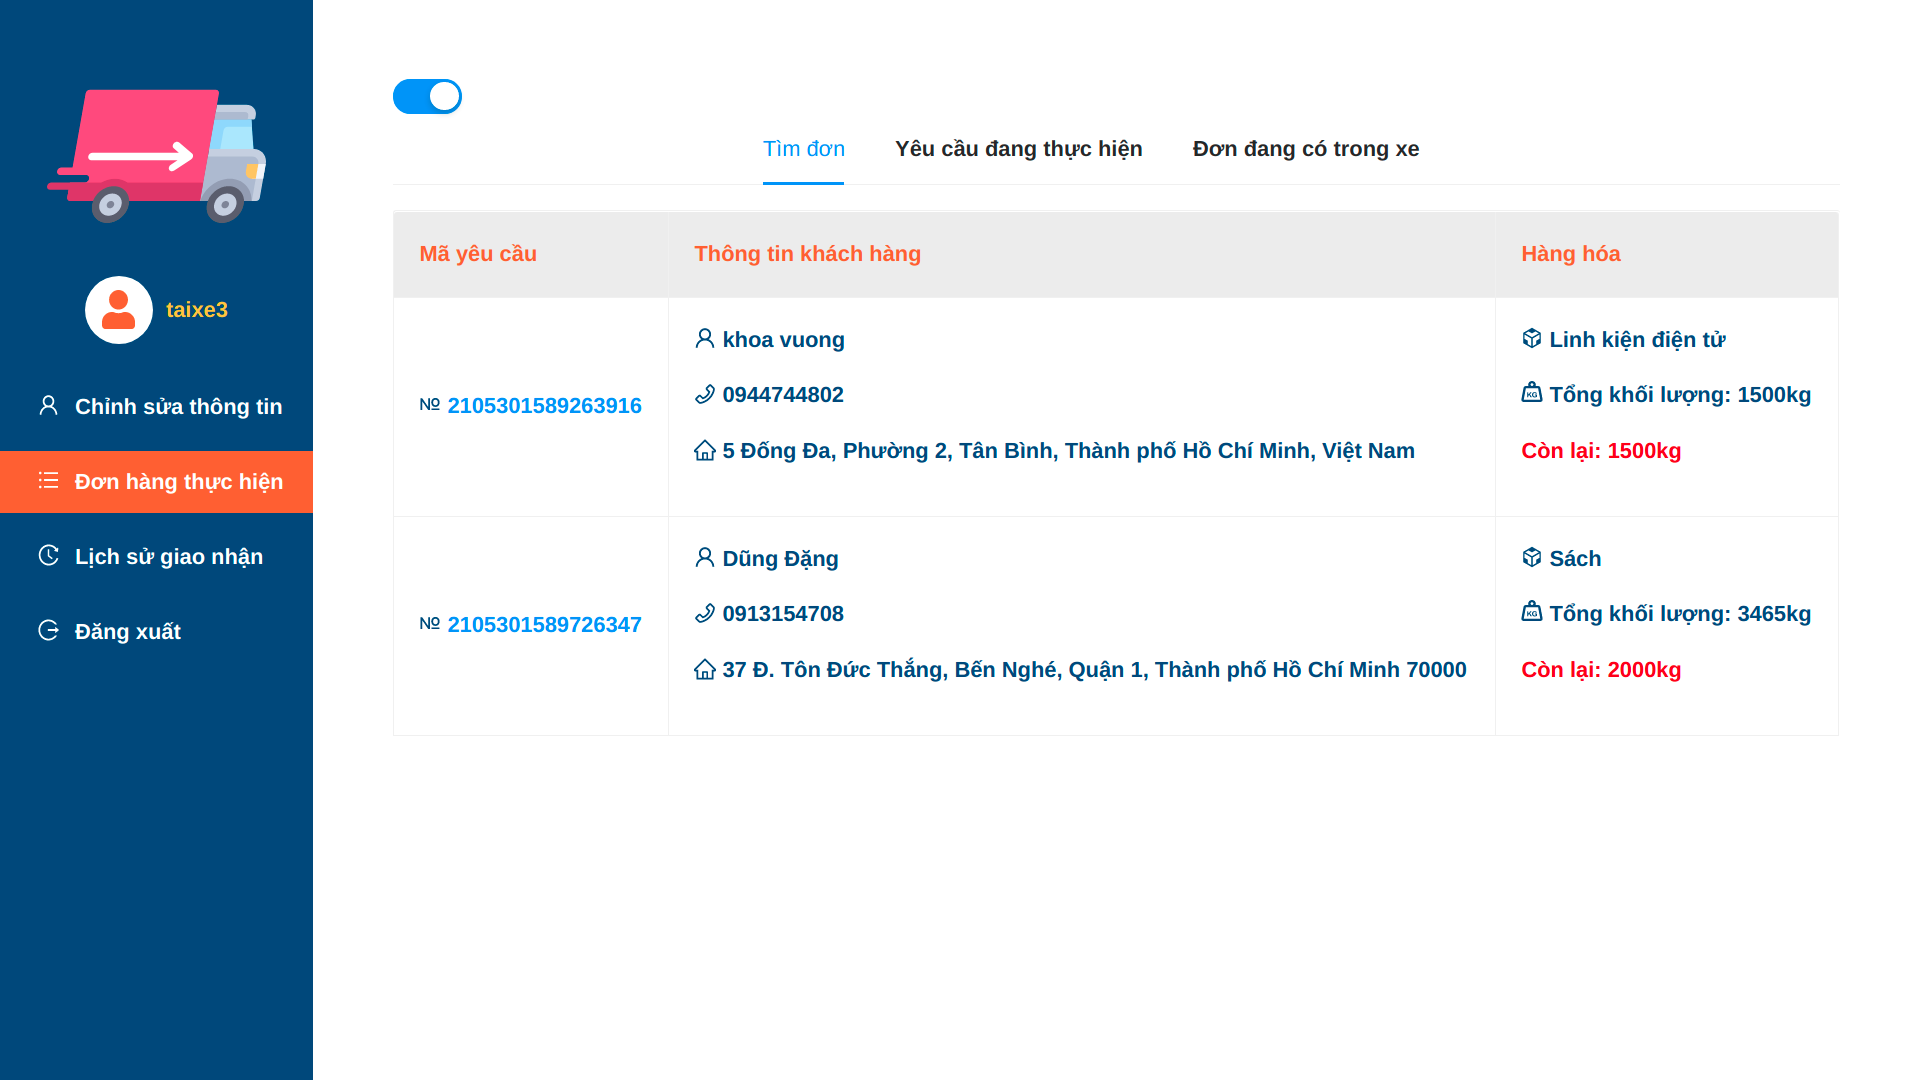
\includegraphics[width=0.8\textwidth]{/driver/driver_find_order.png}
					\centering
					\caption{Giao diện tìm những yêu cầu được gán}
				\end{figure}
			
				\begin{figure}[H]
					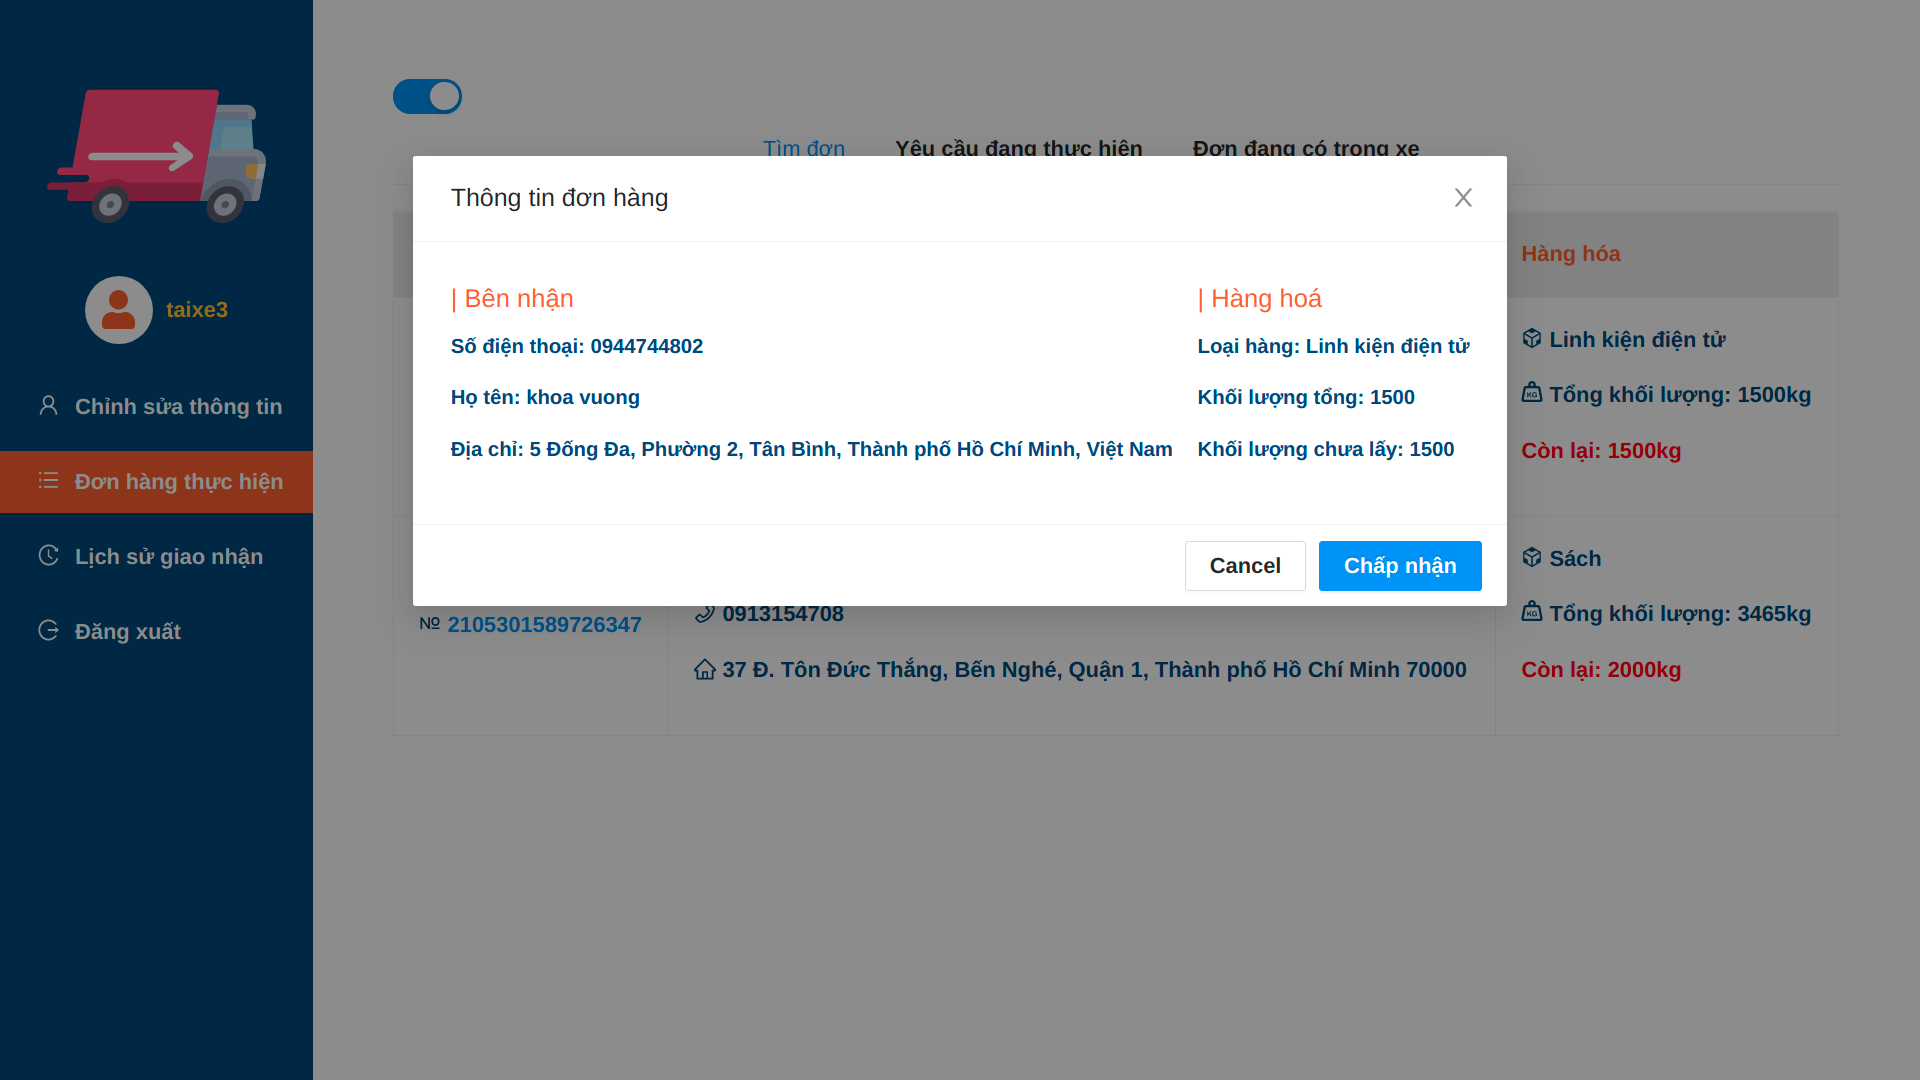
\includegraphics[width=0.8\textwidth]{/driver/driver_find_modal.png}
					\centering
					\caption{Giao diện xác nhận lại thông tin yêu cầu muốn nhận}
				\end{figure}
			
			\subsection{Xem thông tin đơn hàng đang đến lấy}
				\begin{figure}[H]
					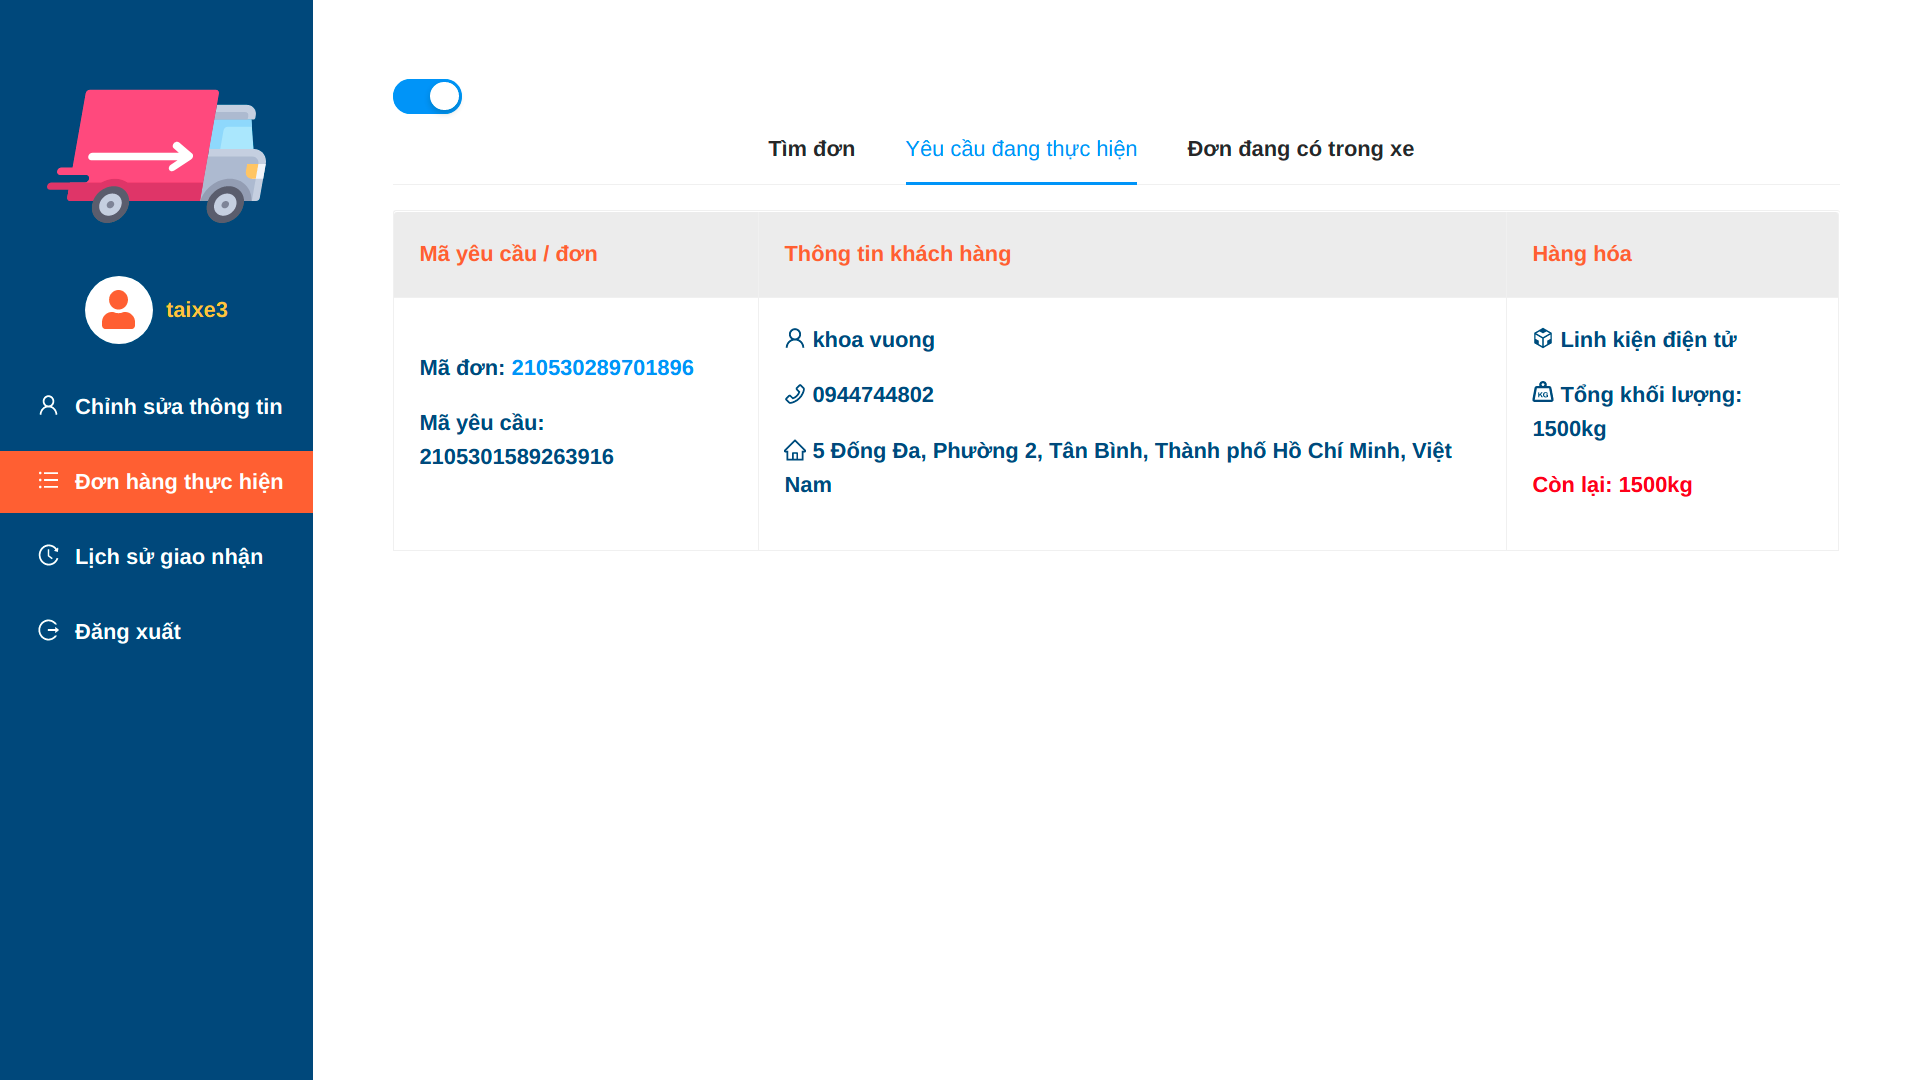
\includegraphics[width=0.8\textwidth]{/driver/driver_current_order.png}
					\centering
					\caption{Giao diện xem thông tin đơn hàng đang đến lấy}
				\end{figure}
				
				\begin{figure}[H]
					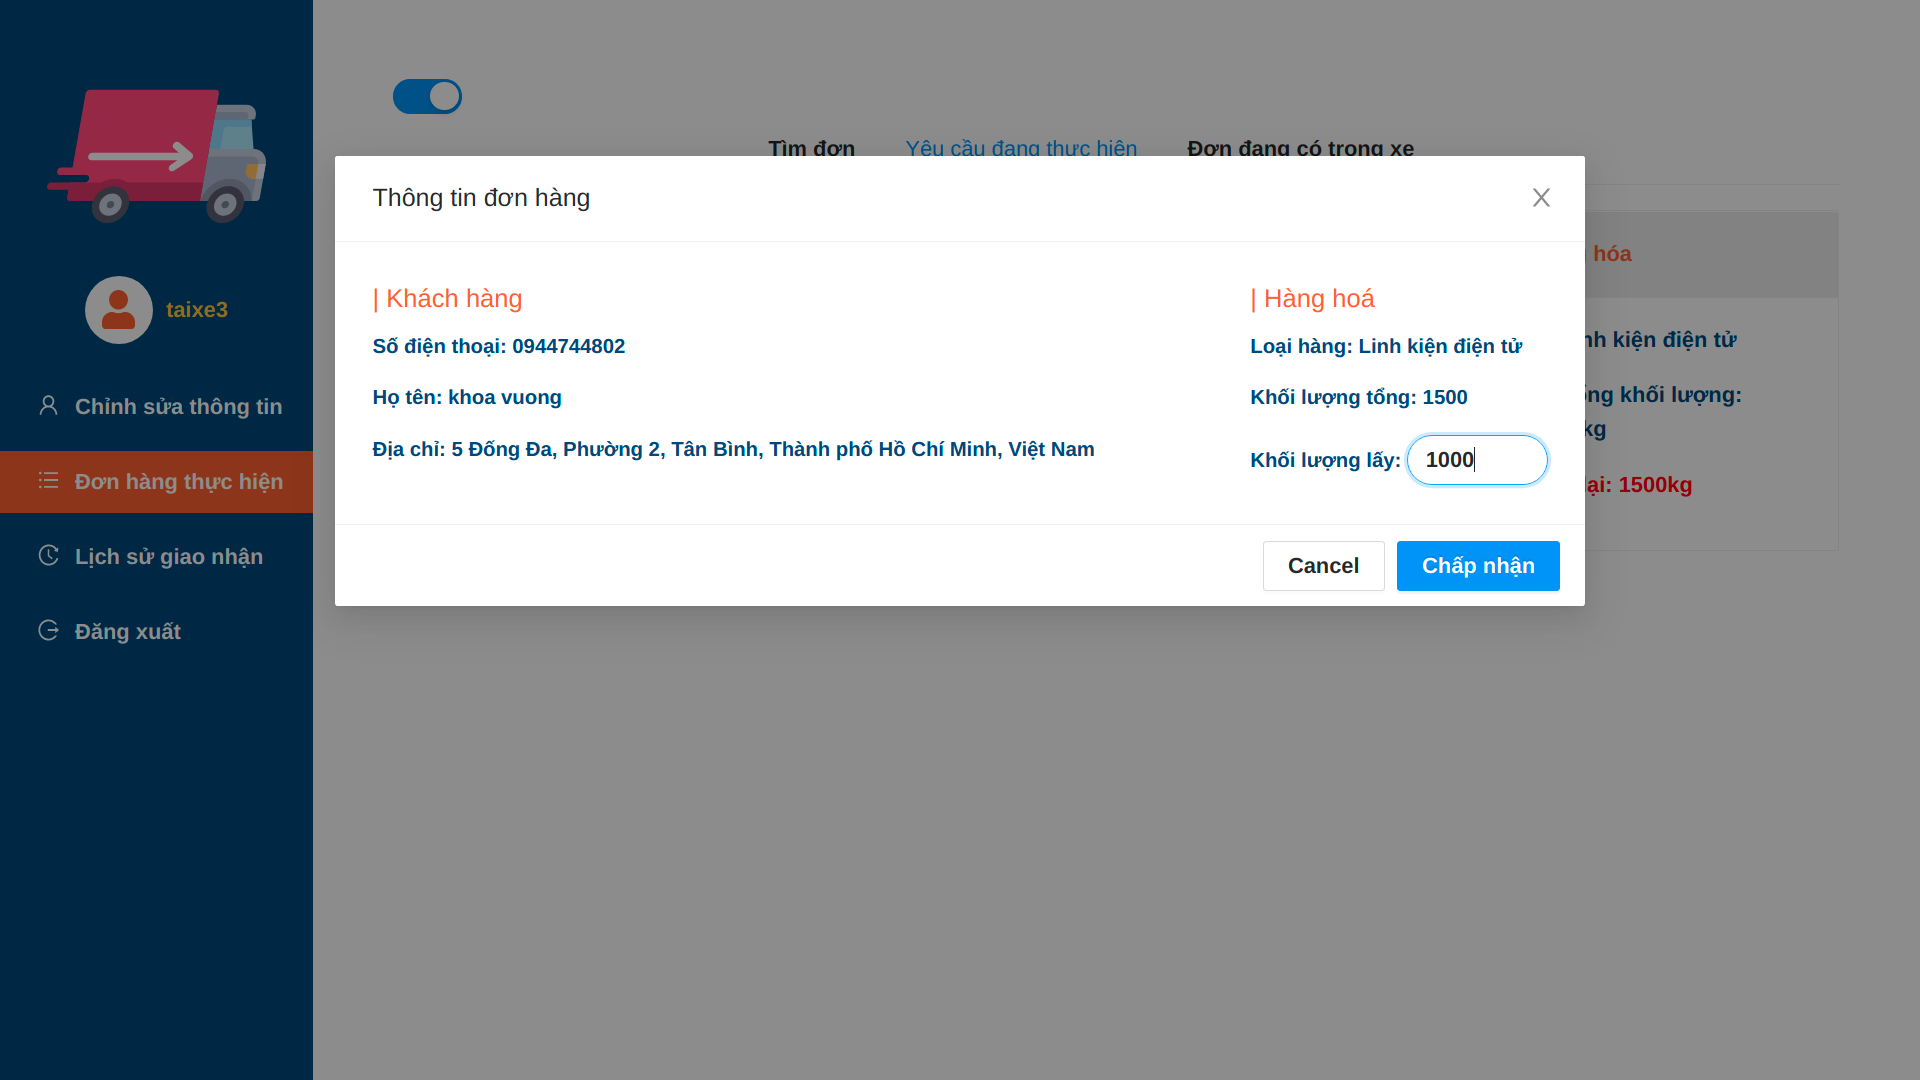
\includegraphics[width=0.8\textwidth]{/driver/driver_current_modal.png}
					\centering
					\caption{Giao diện xác nhận lại thông tin đơn hàng đang muốn nhận}
				\end{figure}
			
			\subsection{Xem thông tin các đơn hàng đang ở trong xe}
				\begin{figure}[H]
					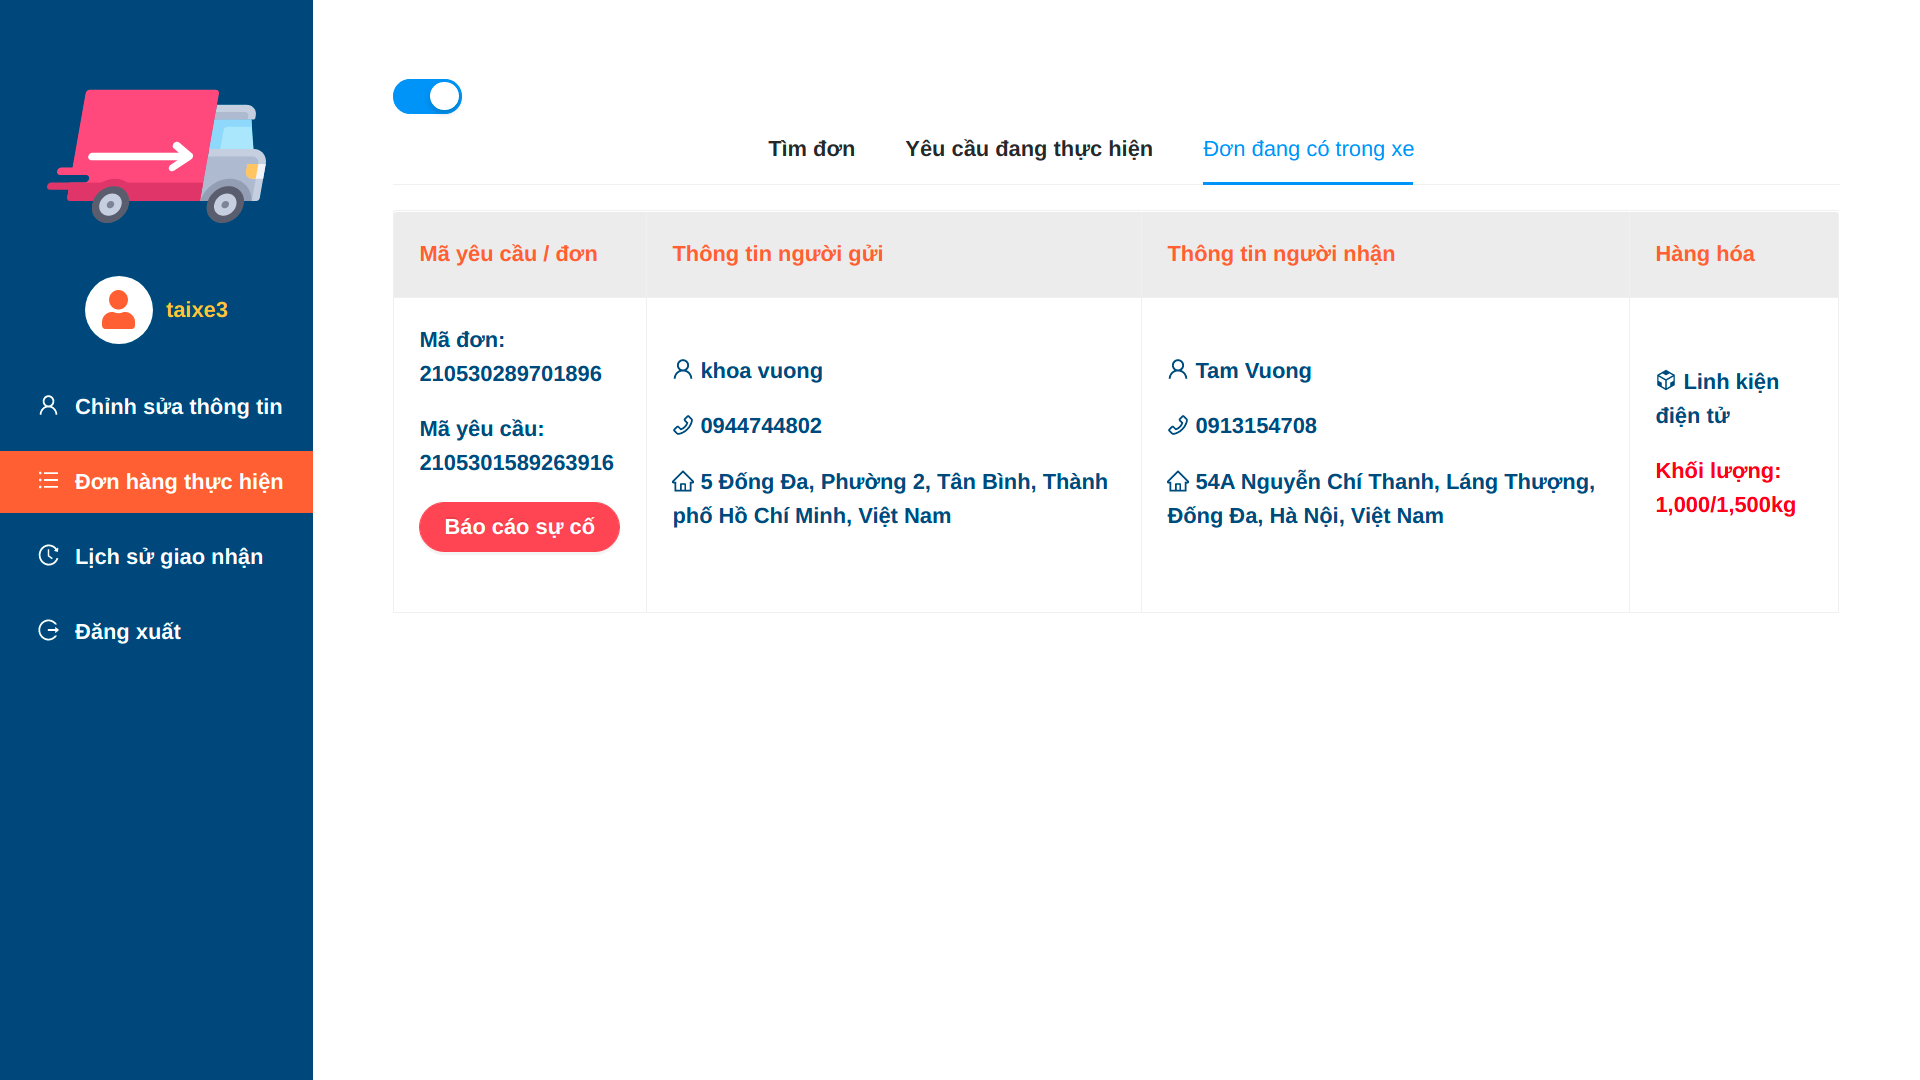
\includegraphics[width=0.8\textwidth]{/driver/driver_intruck.png}
					\centering
					\caption{Giao diện xem thông tin các đơn hàng đang ở trong xe}
				\end{figure}
			
				\begin{figure}[H]
					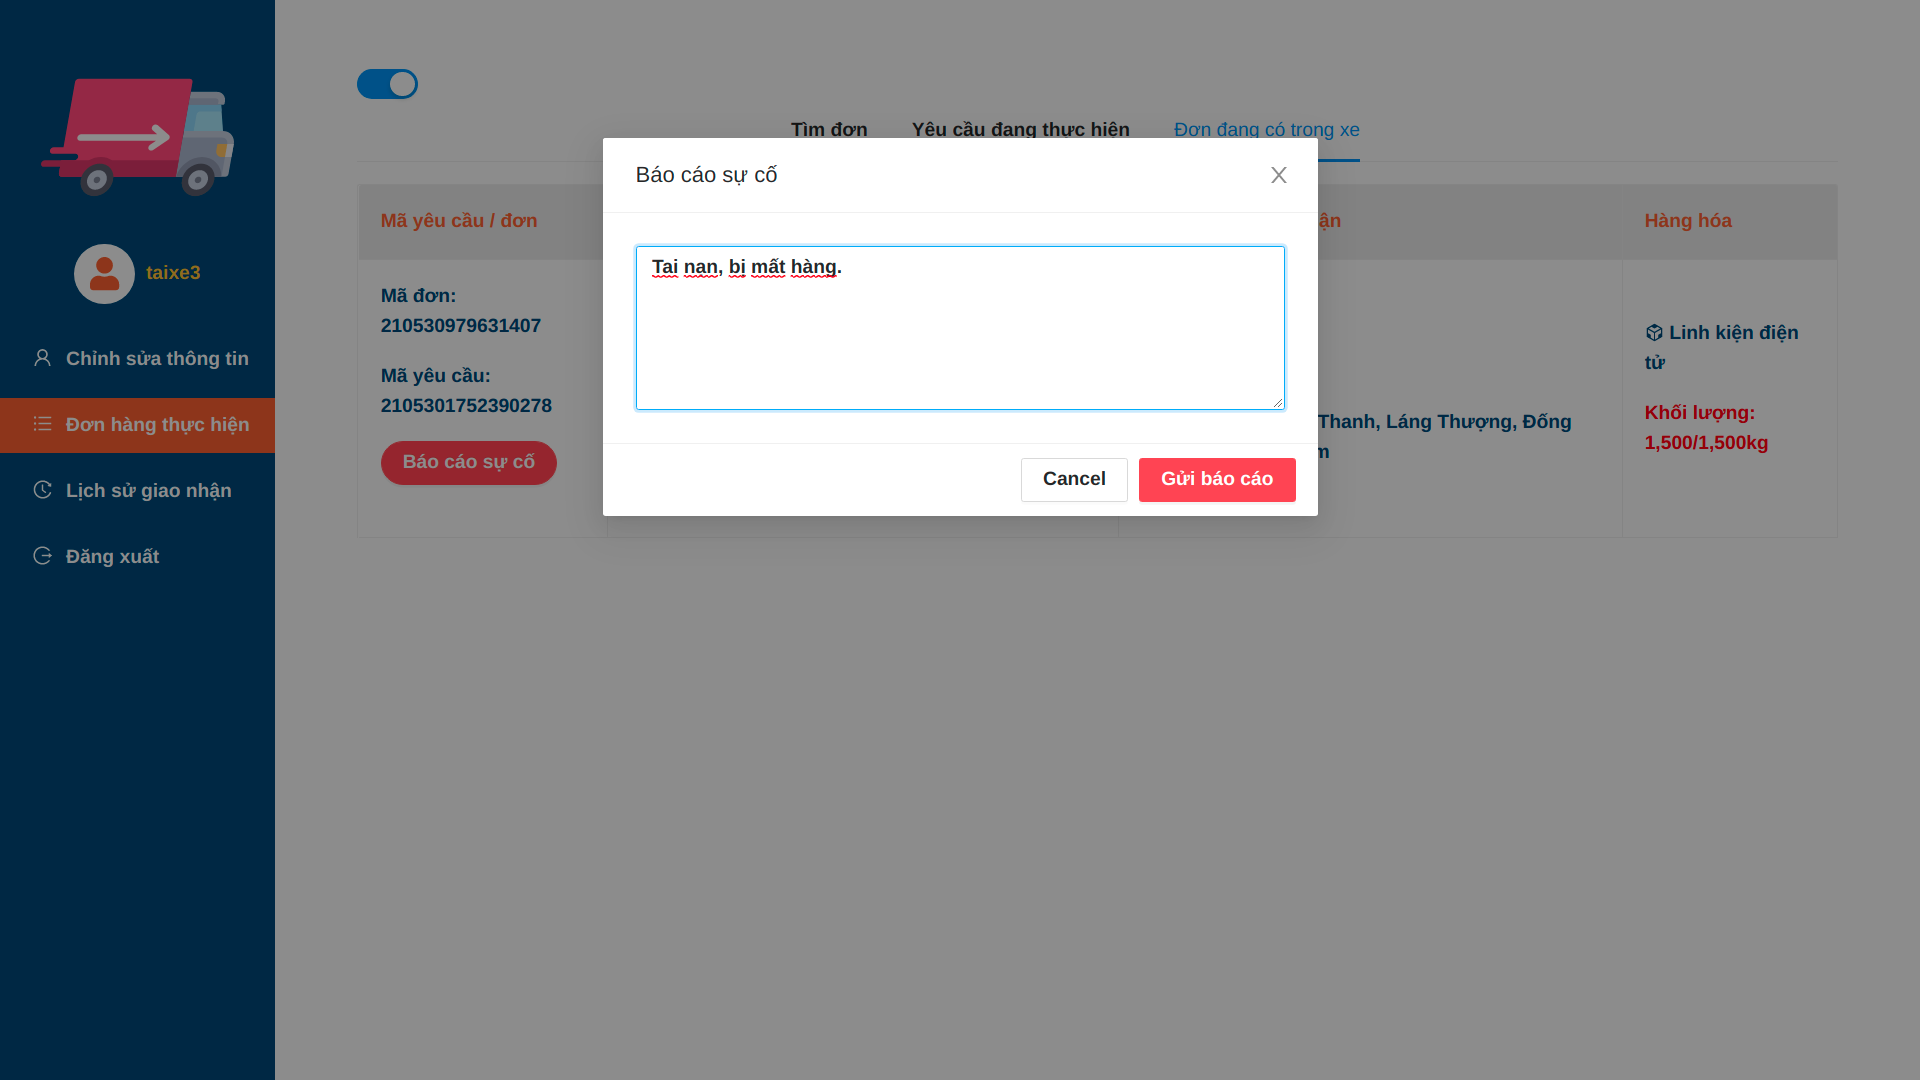
\includegraphics[width=0.8\textwidth]{/driver/driver_issue.png}
					\centering
					\caption{Giao diện báo cáo vấn đề ghi gặp sự cố}
				\end{figure}
			
			\subsection{Xem lịch sử giao nhận hàng}
				\begin{figure}[H]
					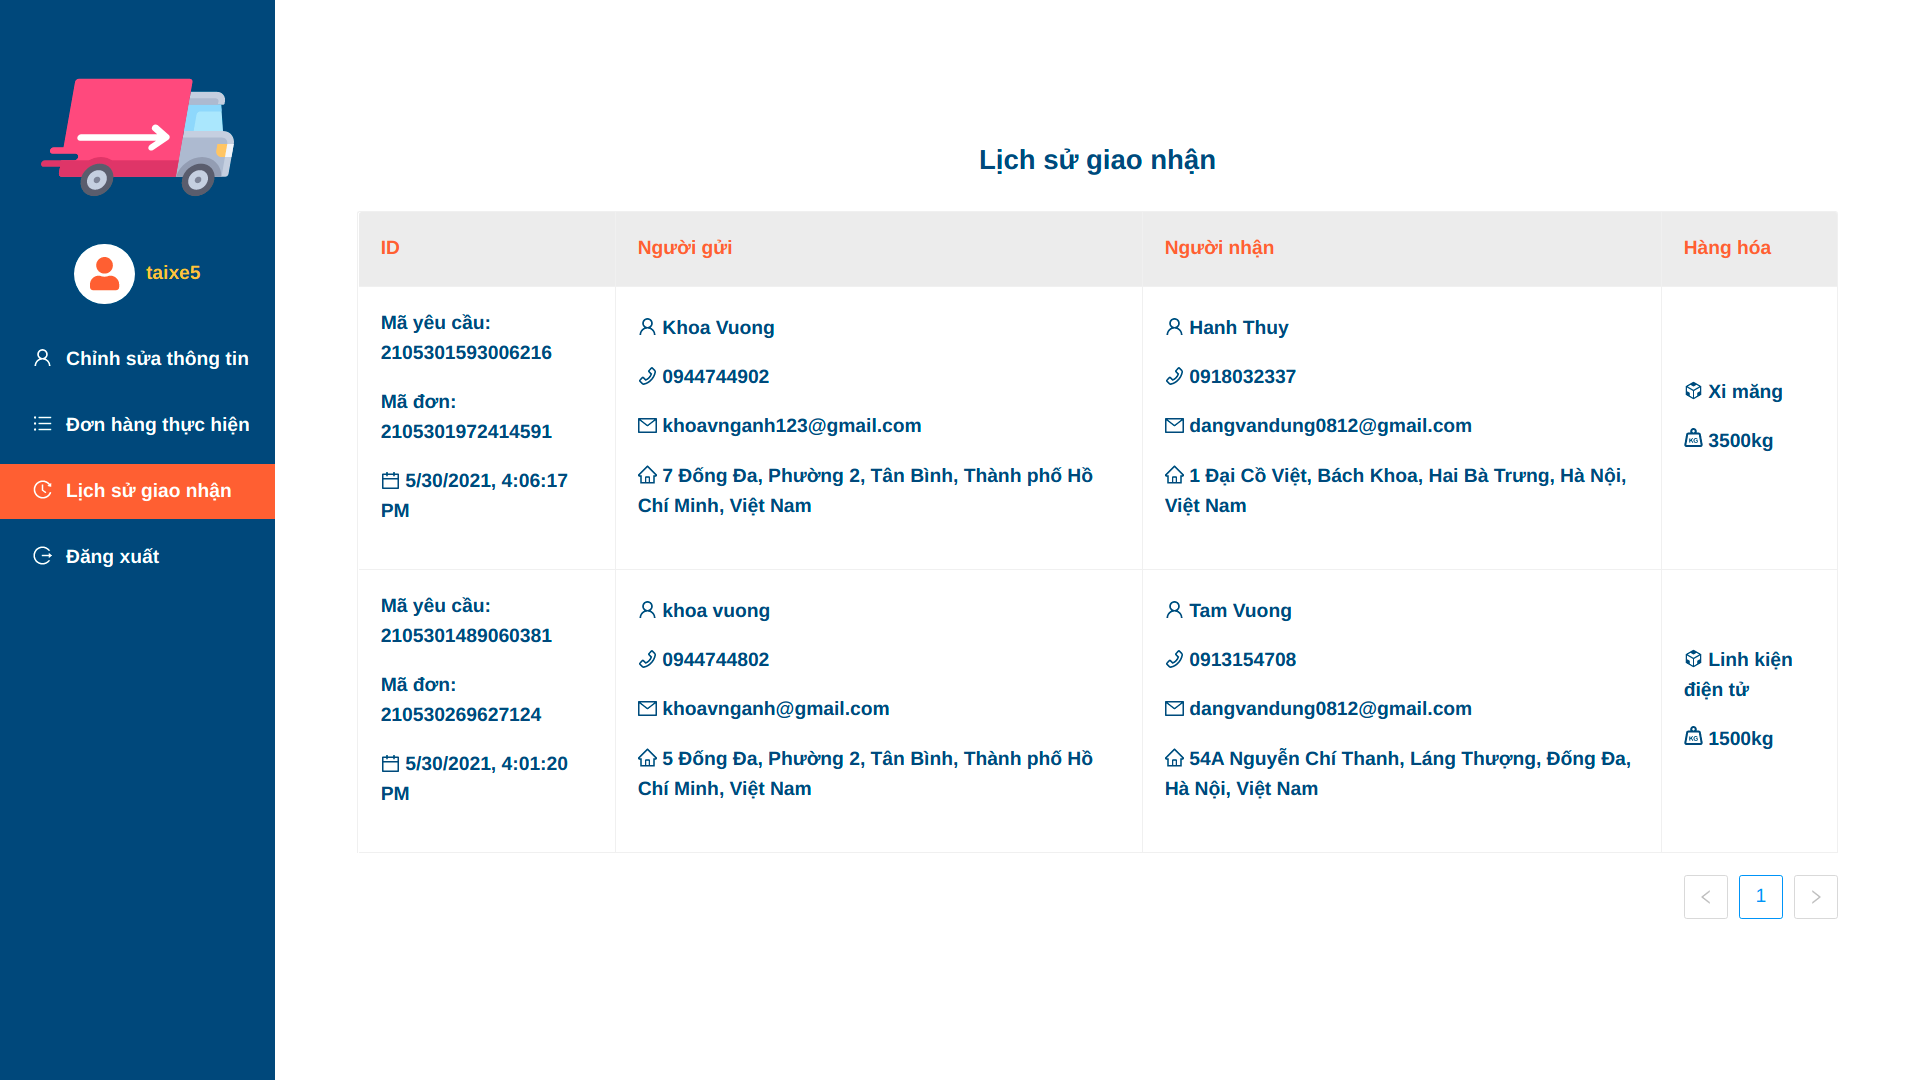
\includegraphics[width=0.8\textwidth]{/driver/driver_history.png}
					\centering
					\caption{Giao diện xem lịch sử giao nhận hàng}
				\end{figure}
			
		\section{Chức năng dành cho thủ kho}
				\begin{figure}[H]
					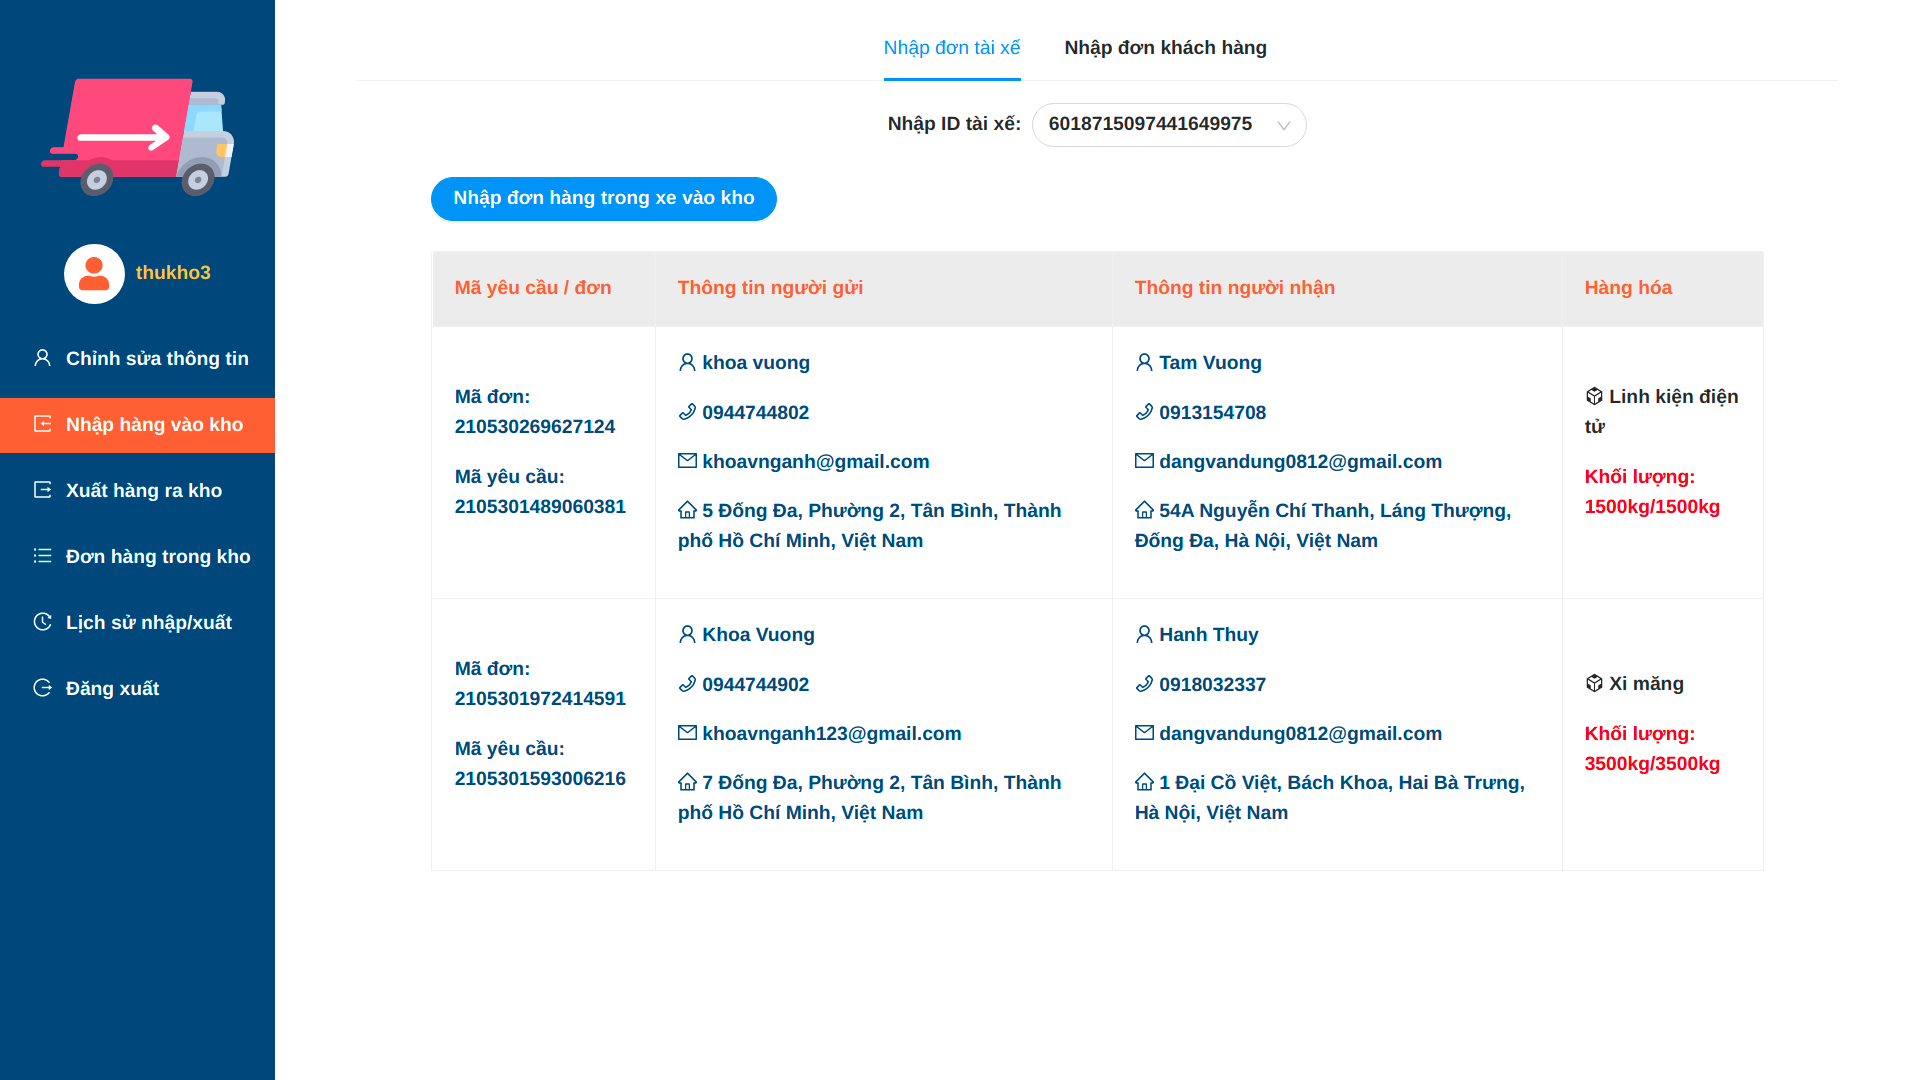
\includegraphics[width=0.8\textwidth]{/stockkeeper/stock_import_driver.png}
					\centering
					\caption{Giao diện nhập ID của tài xế để nhập các đơn hàng trong xe tài xế vào kho}
				\end{figure}
			
				\begin{figure}[H]
					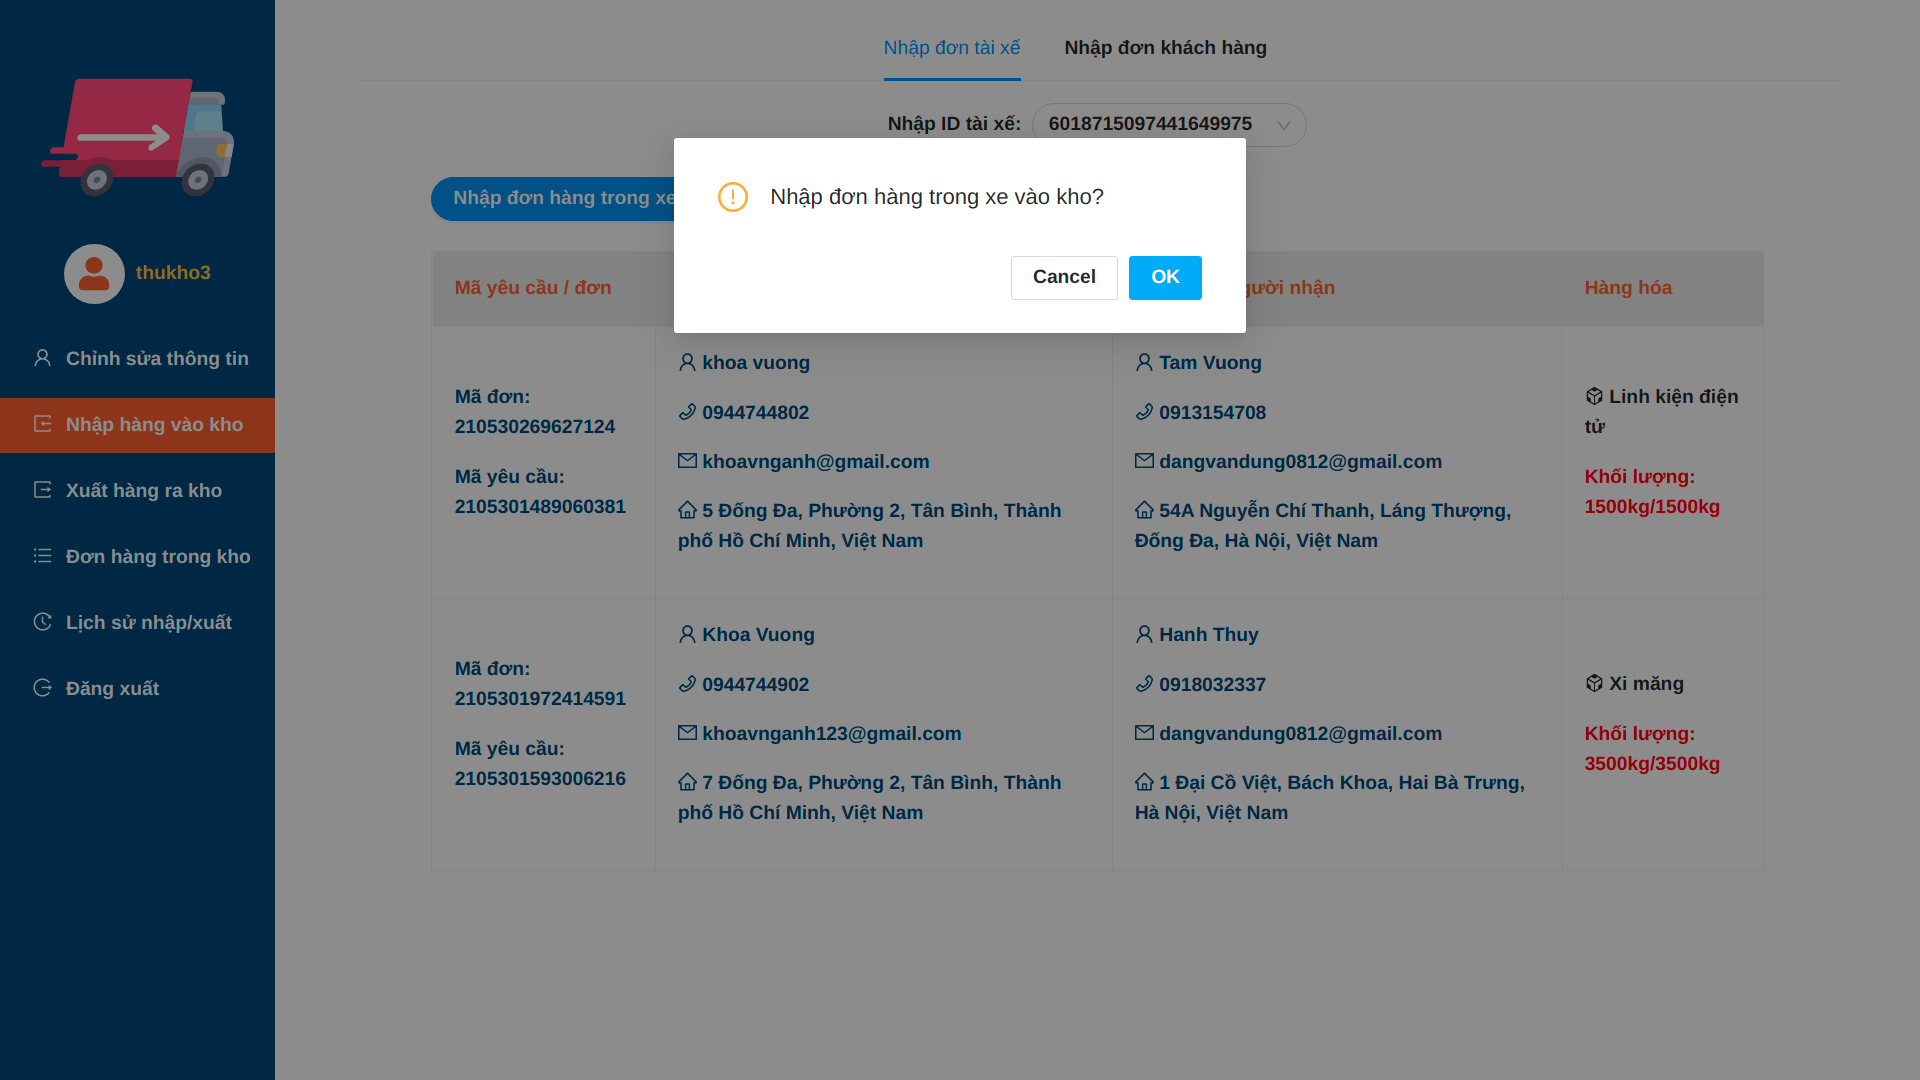
\includegraphics[width=0.8\textwidth]{/stockkeeper/stock_import_driver_prompt.png}
					\centering
					\caption{Xác nhận nhập hàng vào kho}
				\end{figure}
			
				\begin{figure}[H]
					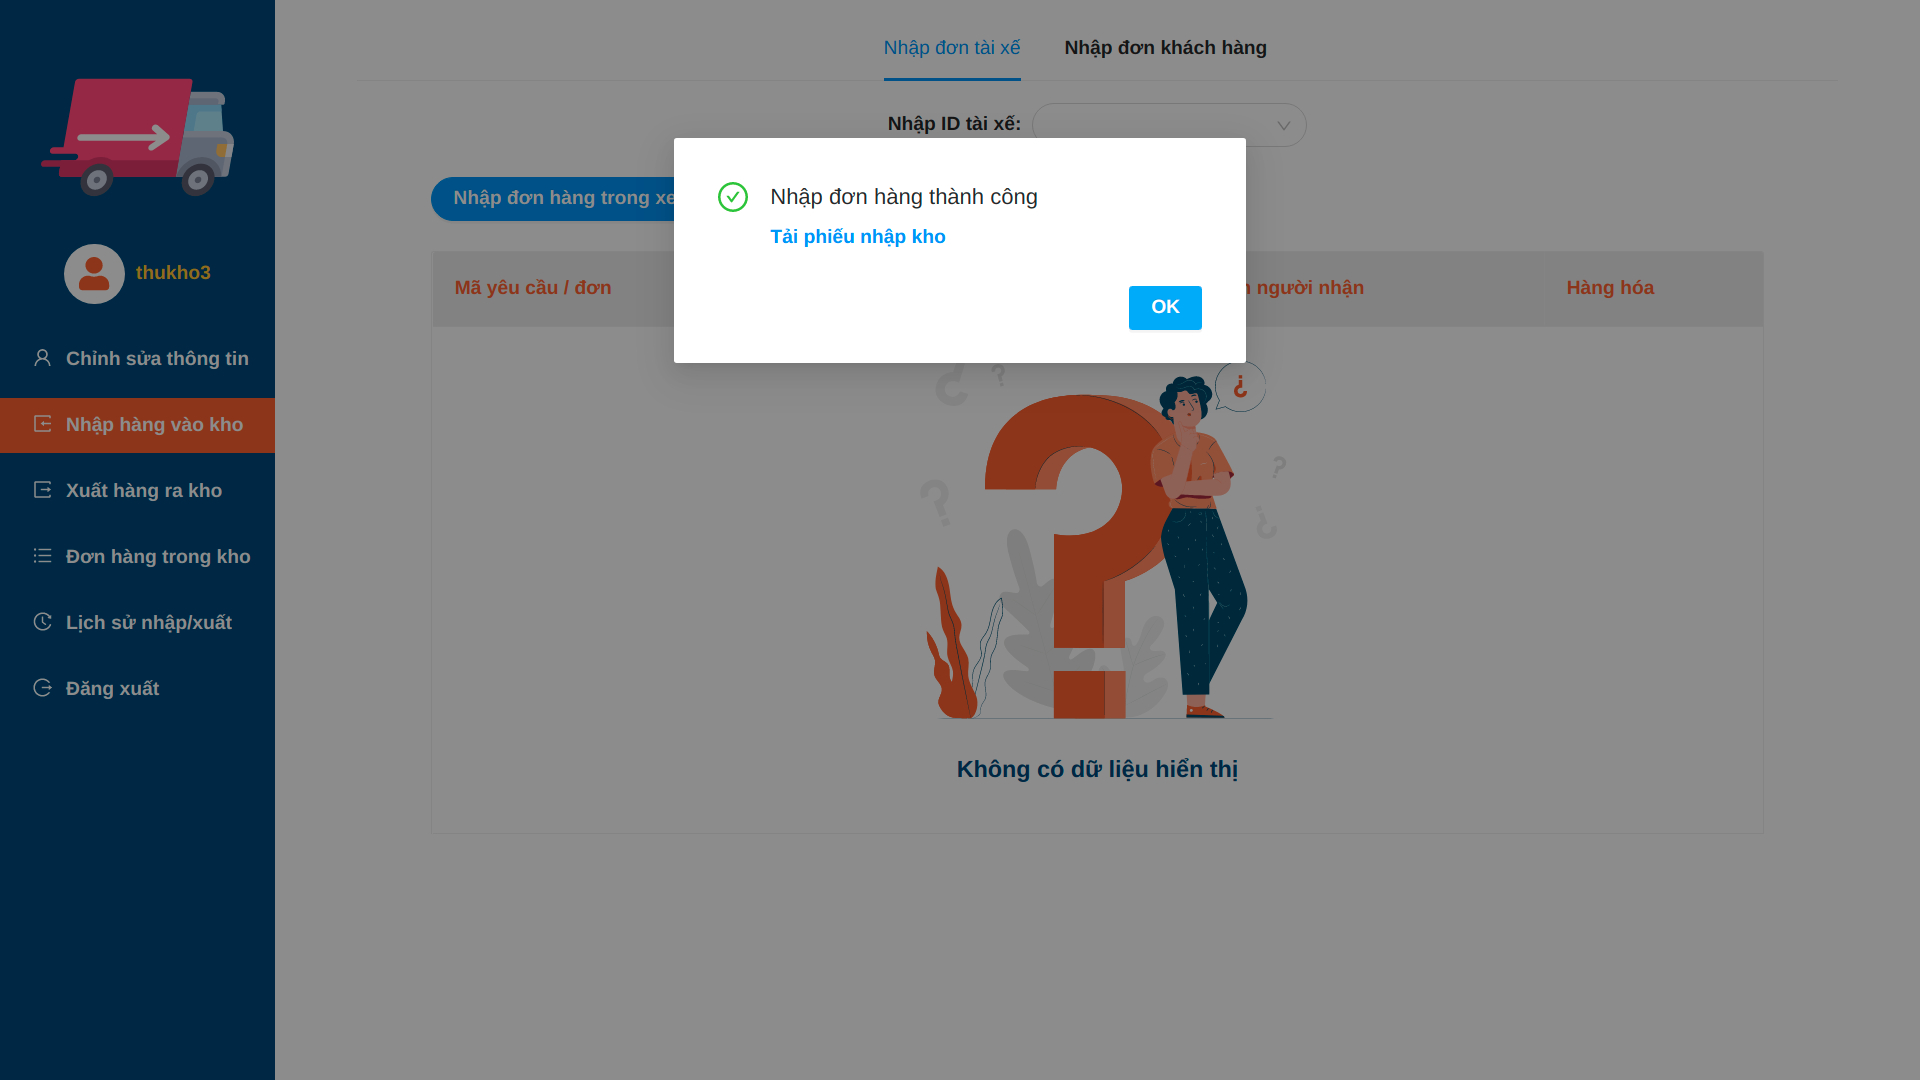
\includegraphics[width=0.8\textwidth]{/stockkeeper/stock_import_driver_pdf.png}
					\centering
					\caption{Nhập hàng thành công và cho thủ kho có thể tài phiếu nhập kho}
				\end{figure}
			
				\begin{figure}[H]
					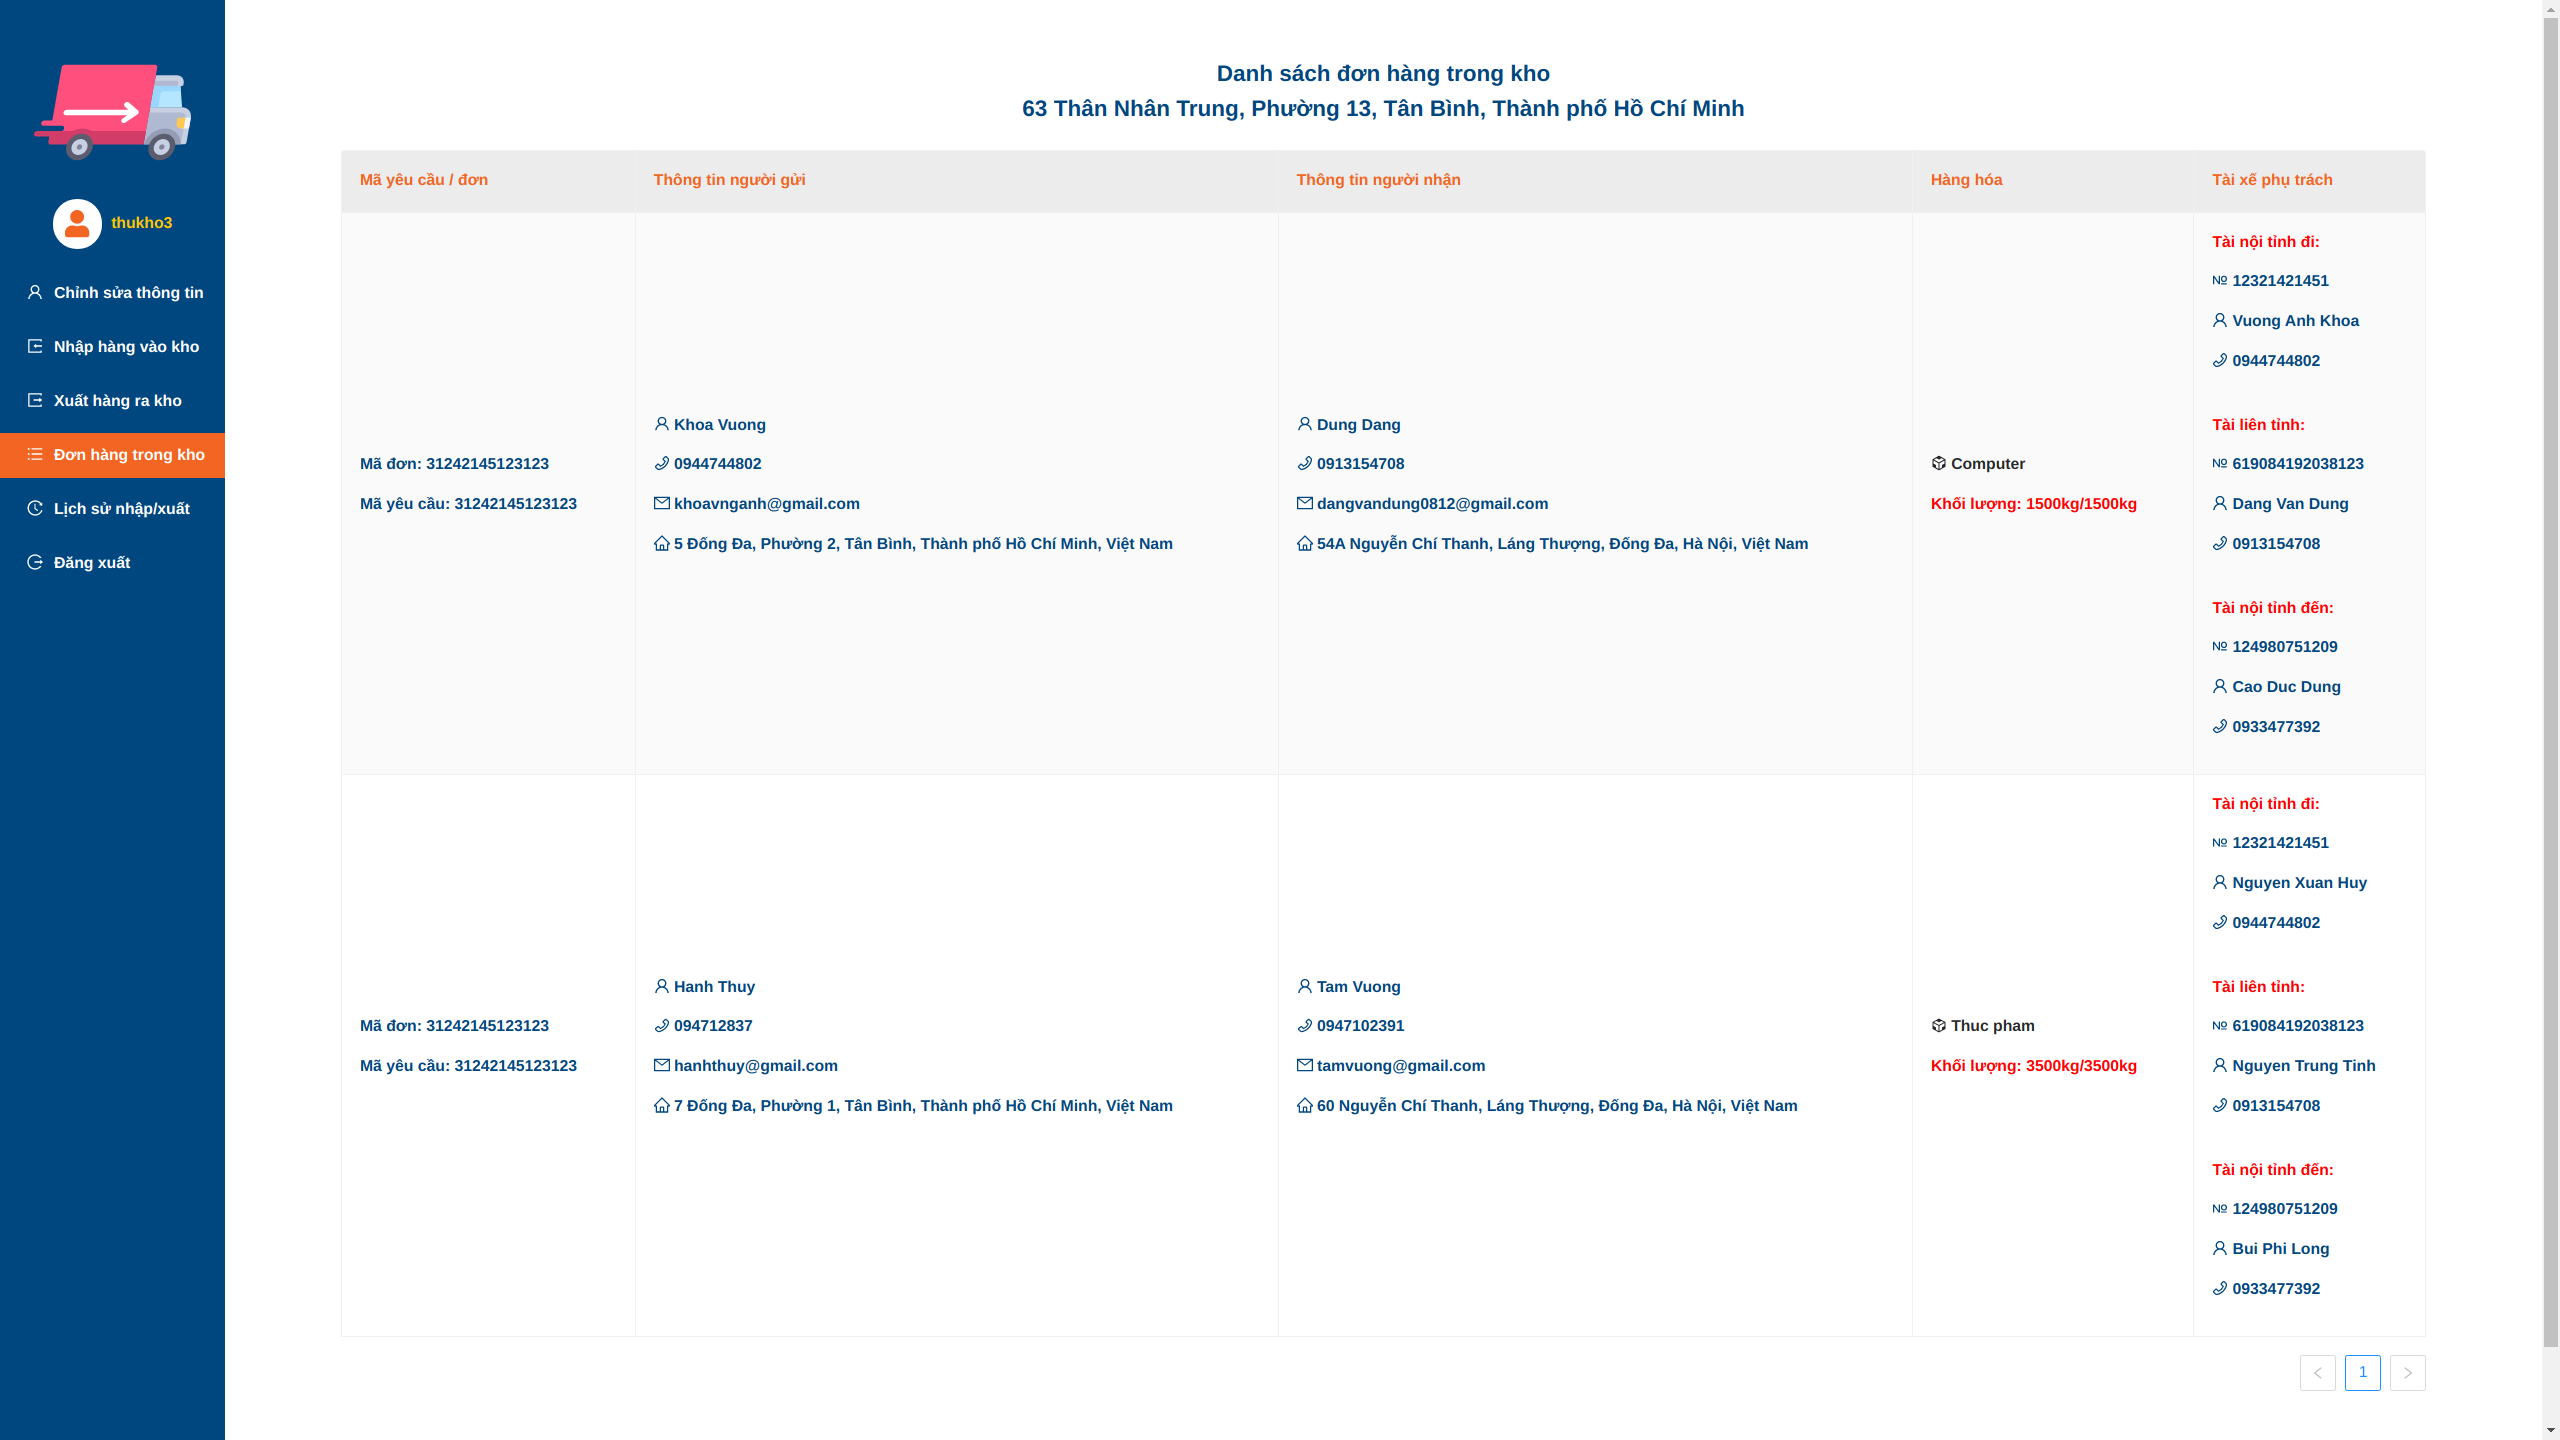
\includegraphics[width=0.8\textwidth]{/stockkeeper/stock_list.png}
					\centering
					\caption{Danh sách các đơn hàng trong kho}
				\end{figure}
			
				\begin{figure}[H]
					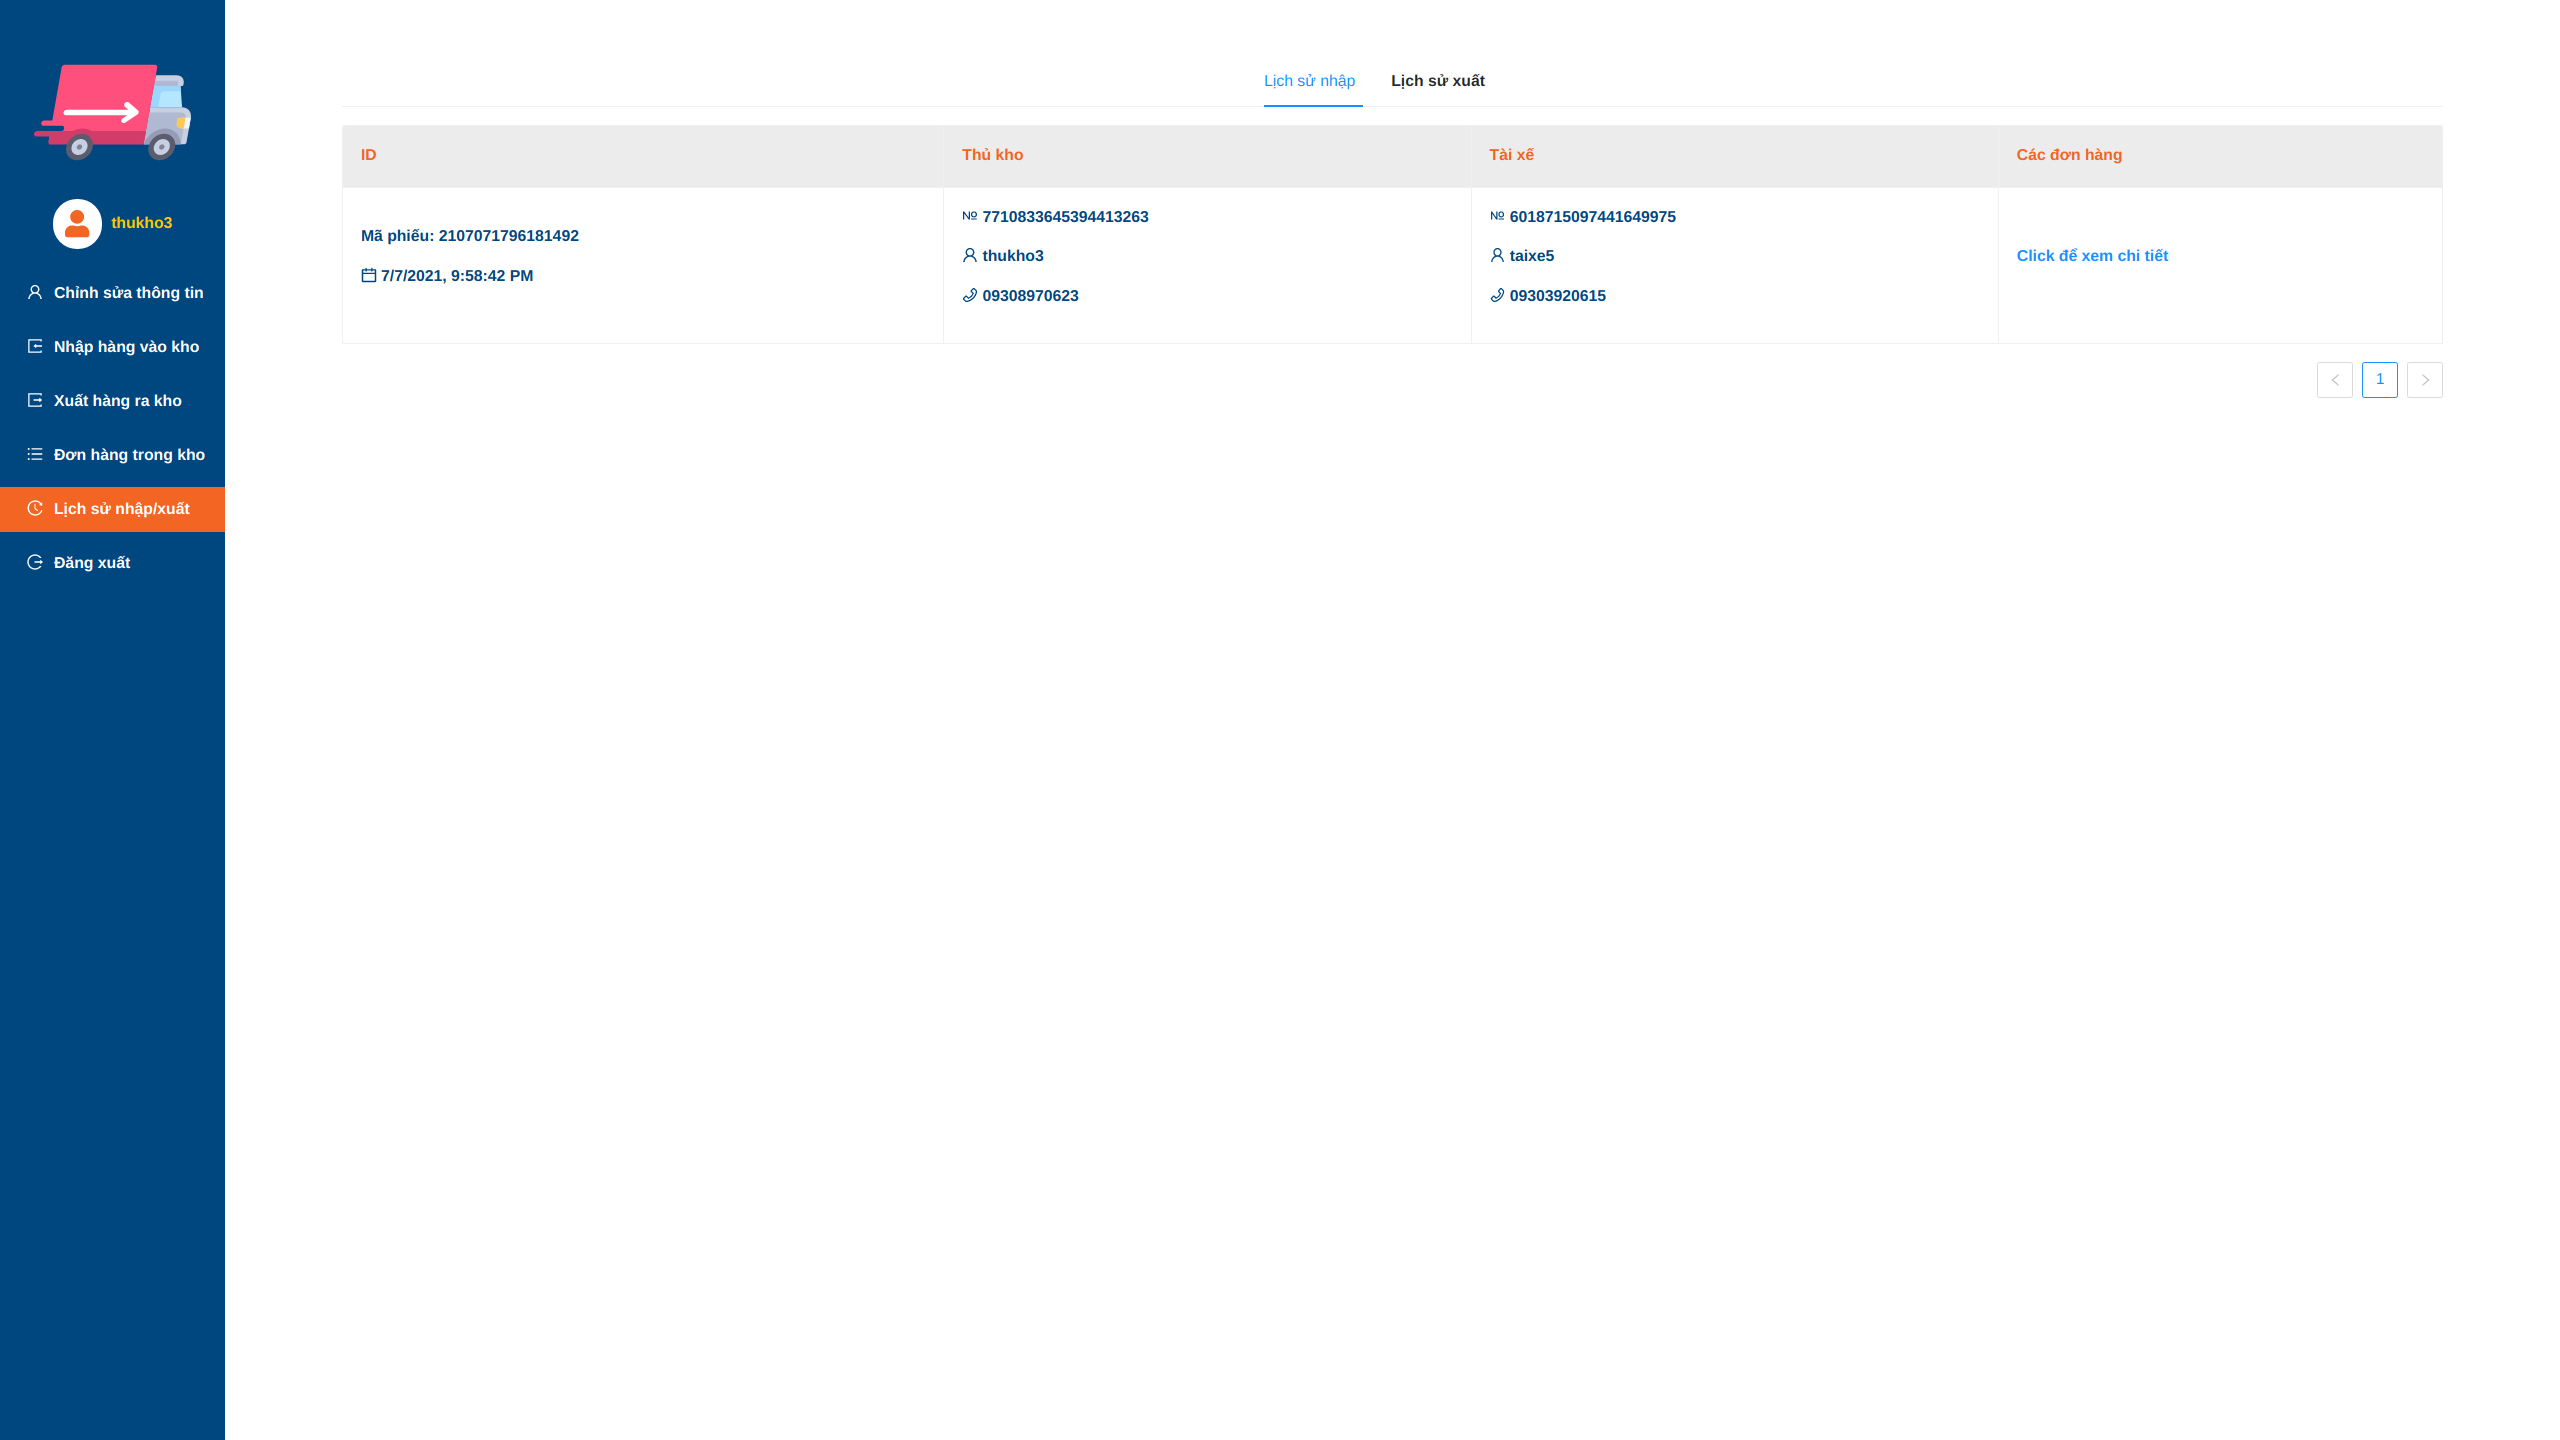
\includegraphics[width=0.8\textwidth]{/stockkeeper/stock_history.png}
					\centering
					\caption{Lịch sử nhập/xuất kho}
				\end{figure}
			
				\begin{figure}[H]
					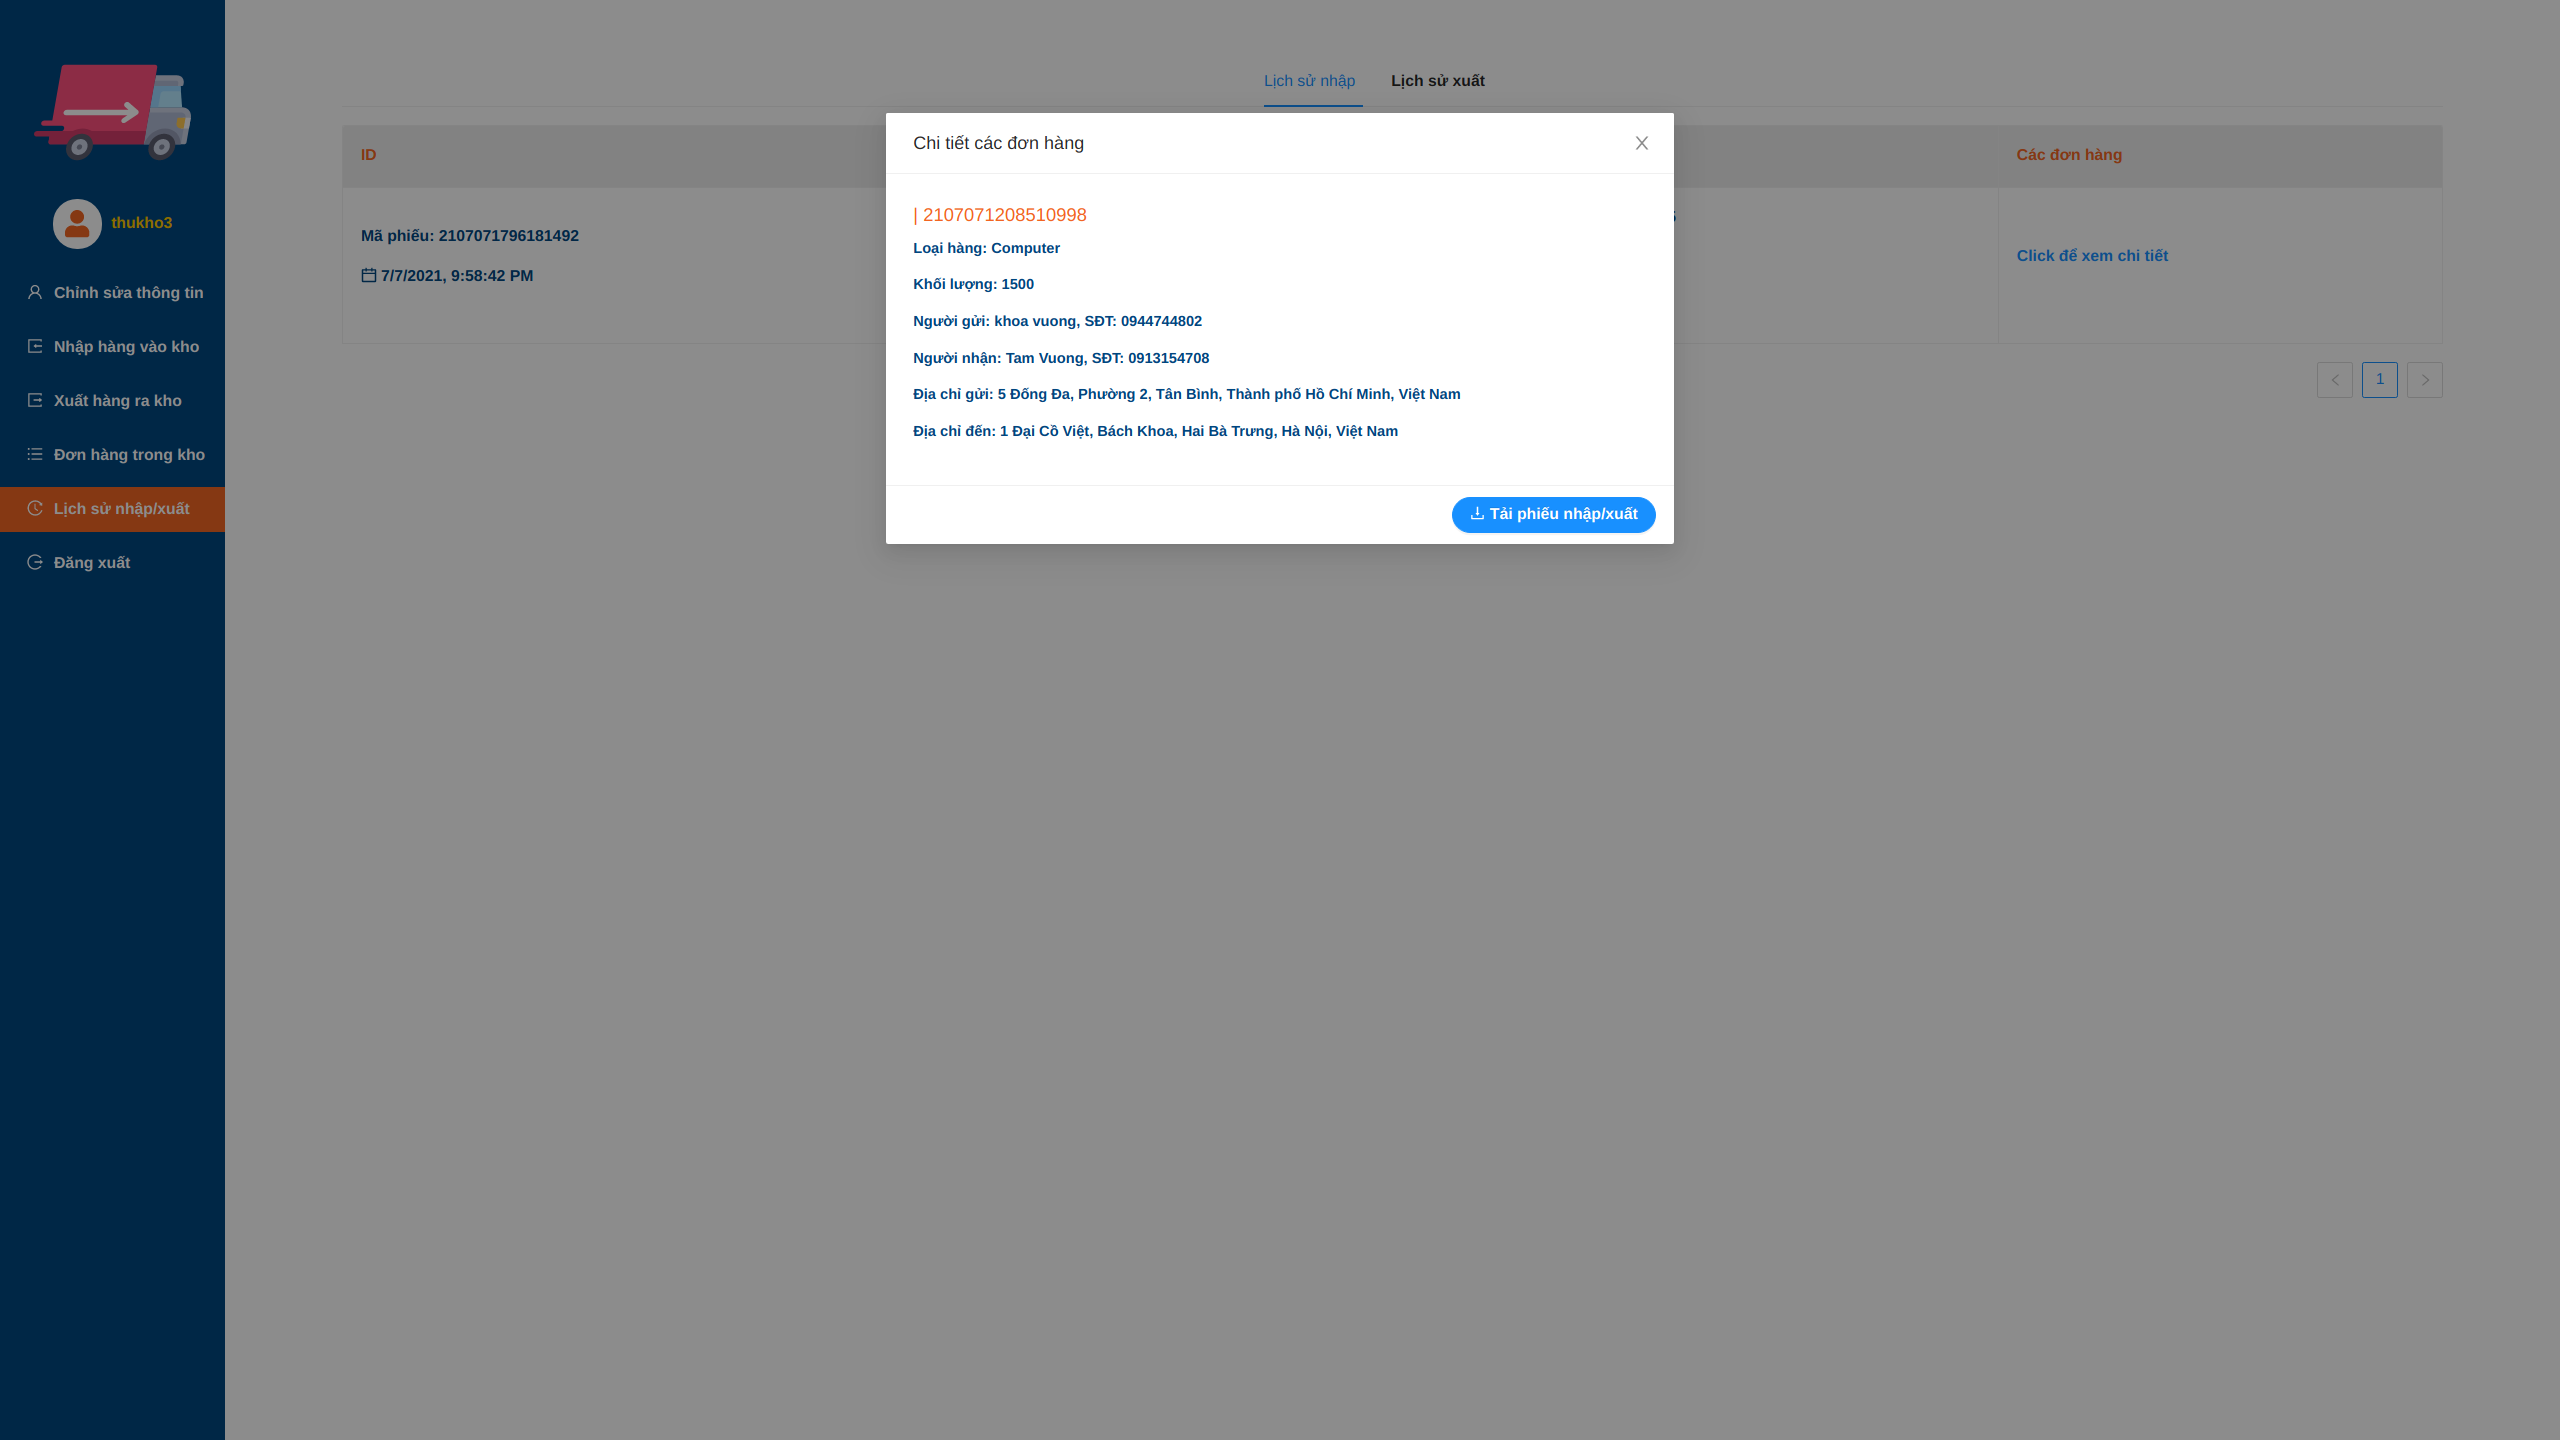
\includegraphics[width=0.8\textwidth]{/stockkeeper/stock_history_detail.png}
					\centering
					\caption{Thông tin chi tiết của một lần nhập/xuất đơn hàng (Cho phép tải pdf về)}
				\end{figure}
			
				\begin{figure}[H]
					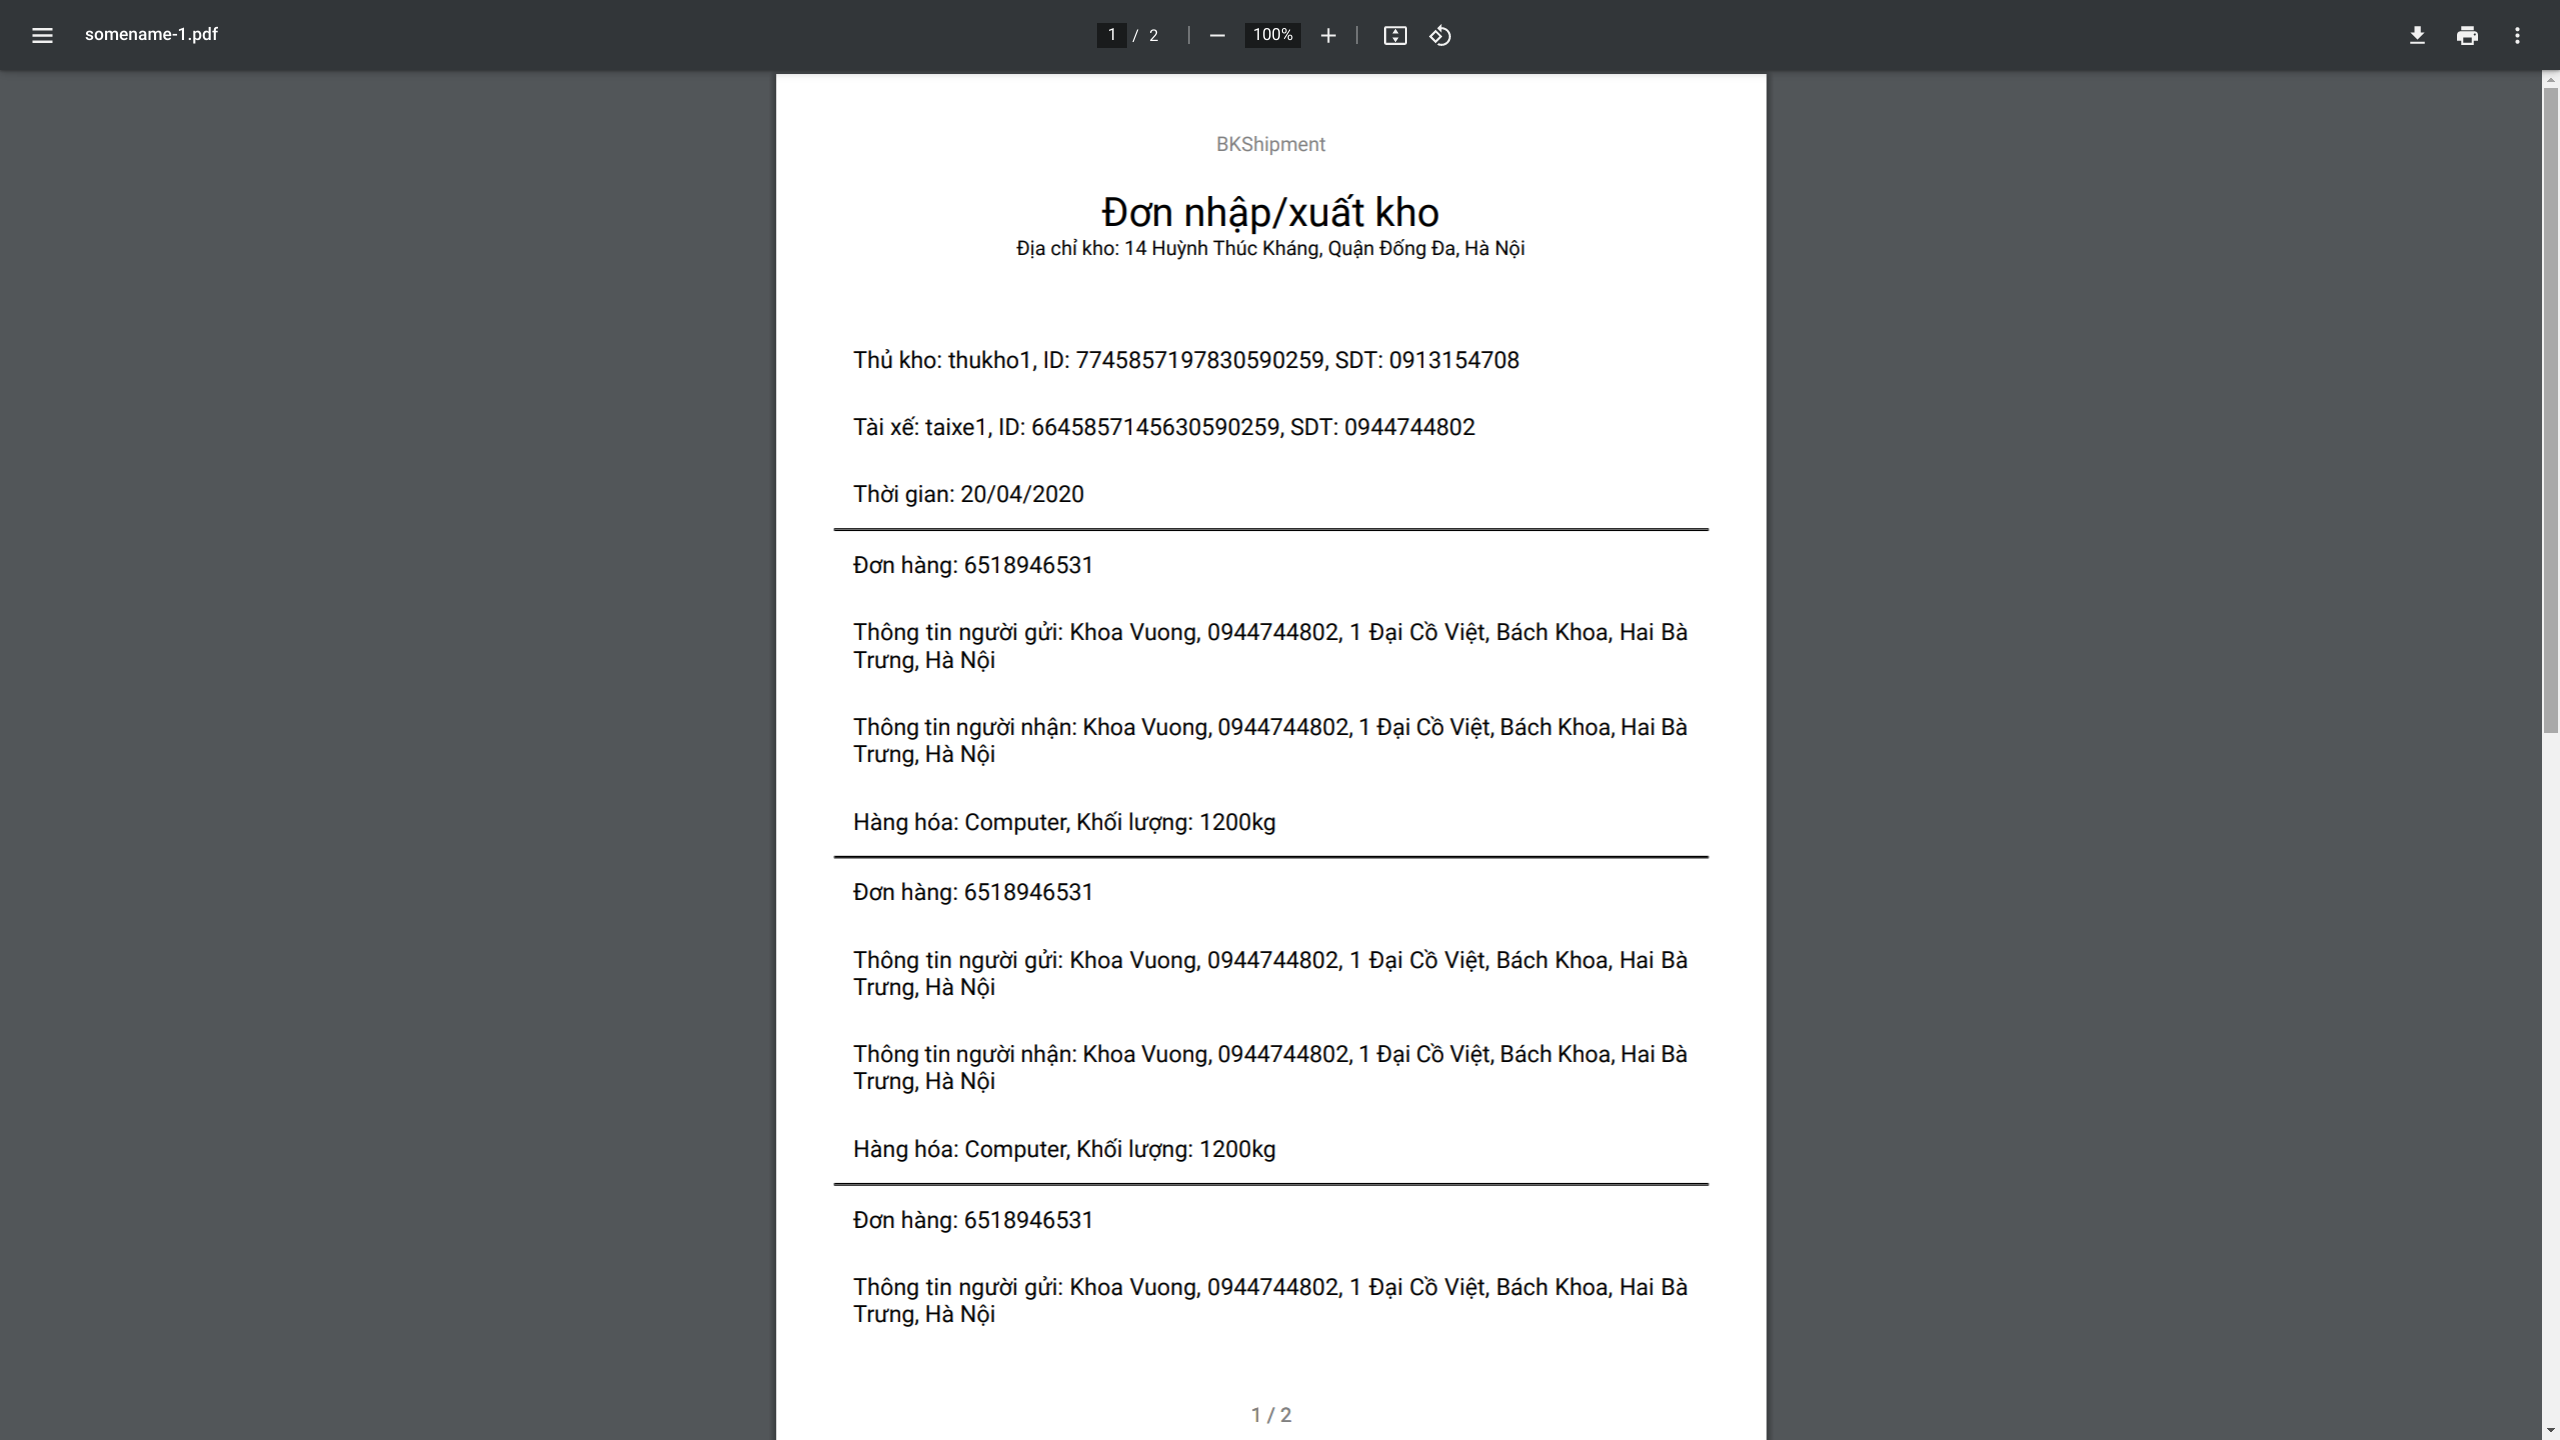
\includegraphics[width=0.8\textwidth]{/stockkeeper/stock_pdf.png}
					\centering
					\caption{Format mẫu của 1 đơn nhập/xuất kho}
				\end{figure}
			
				\begin{figure}[H]
					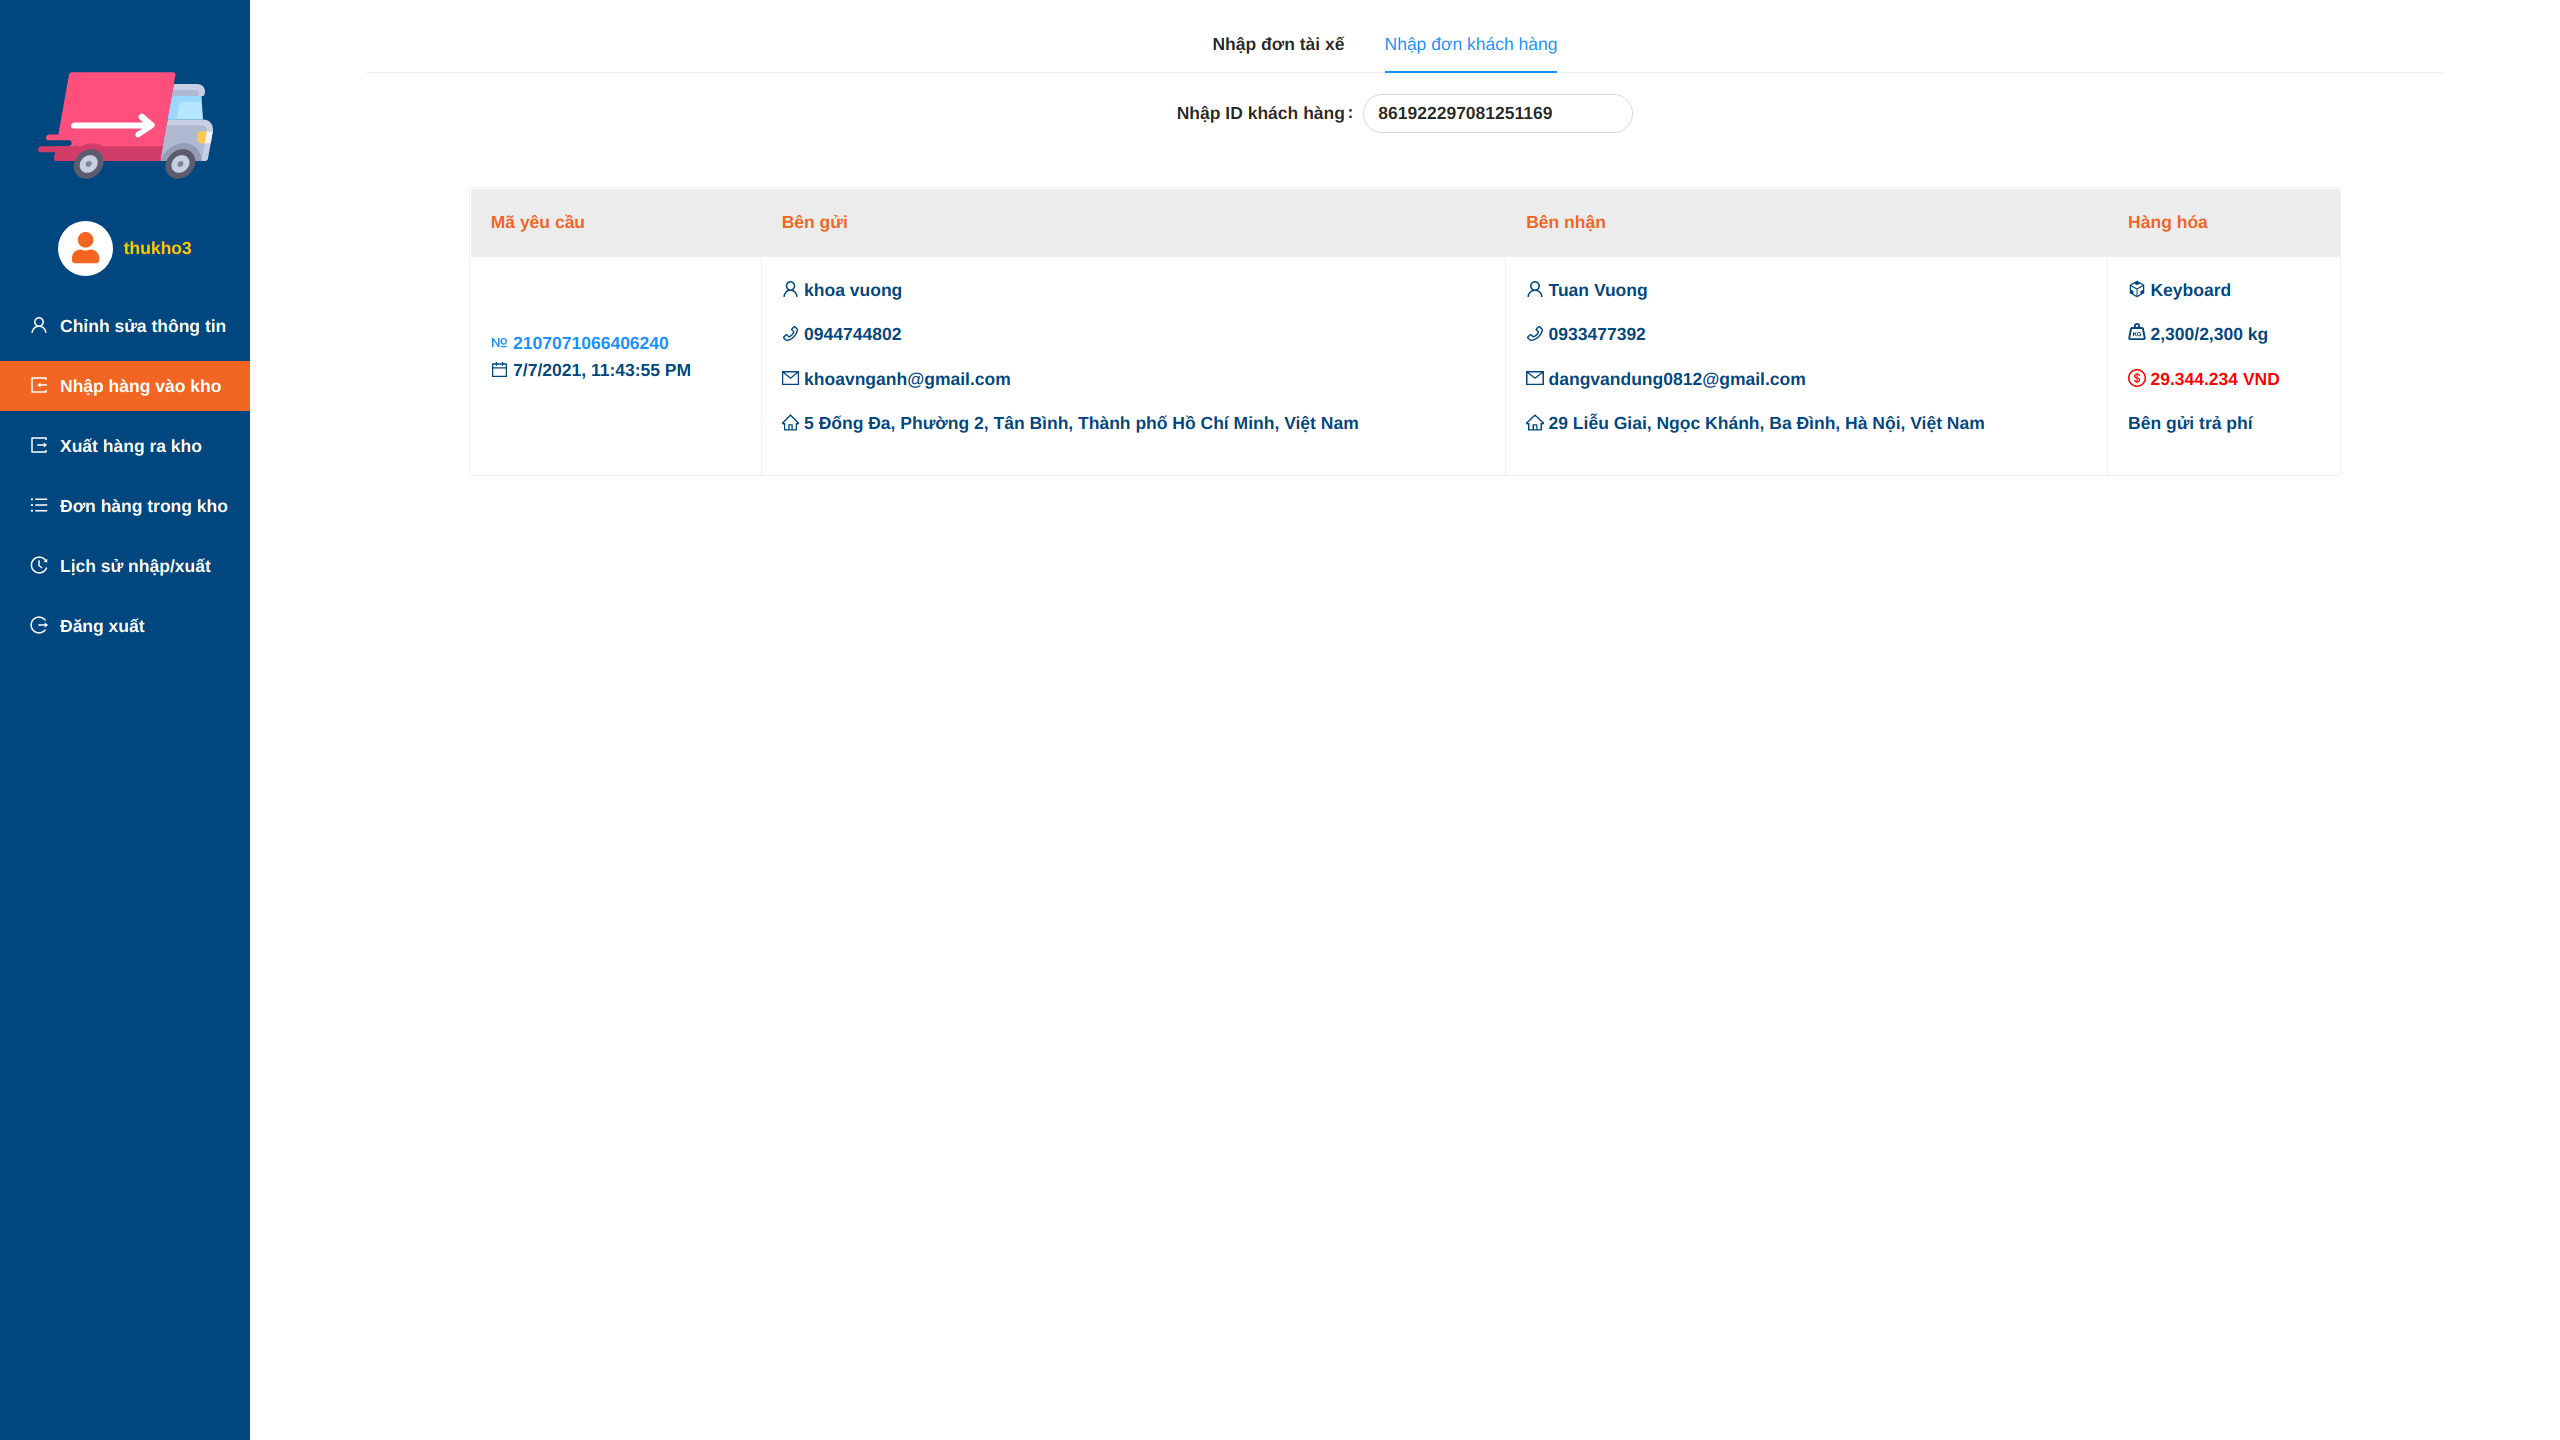
\includegraphics[width=0.8\textwidth]{/stockkeeper/stock_import_customer.png}
					\centering
					\caption{Nhập ID của khách hàng để nhập đơn vào kho}
				\end{figure}
			
				\begin{figure}[H]
					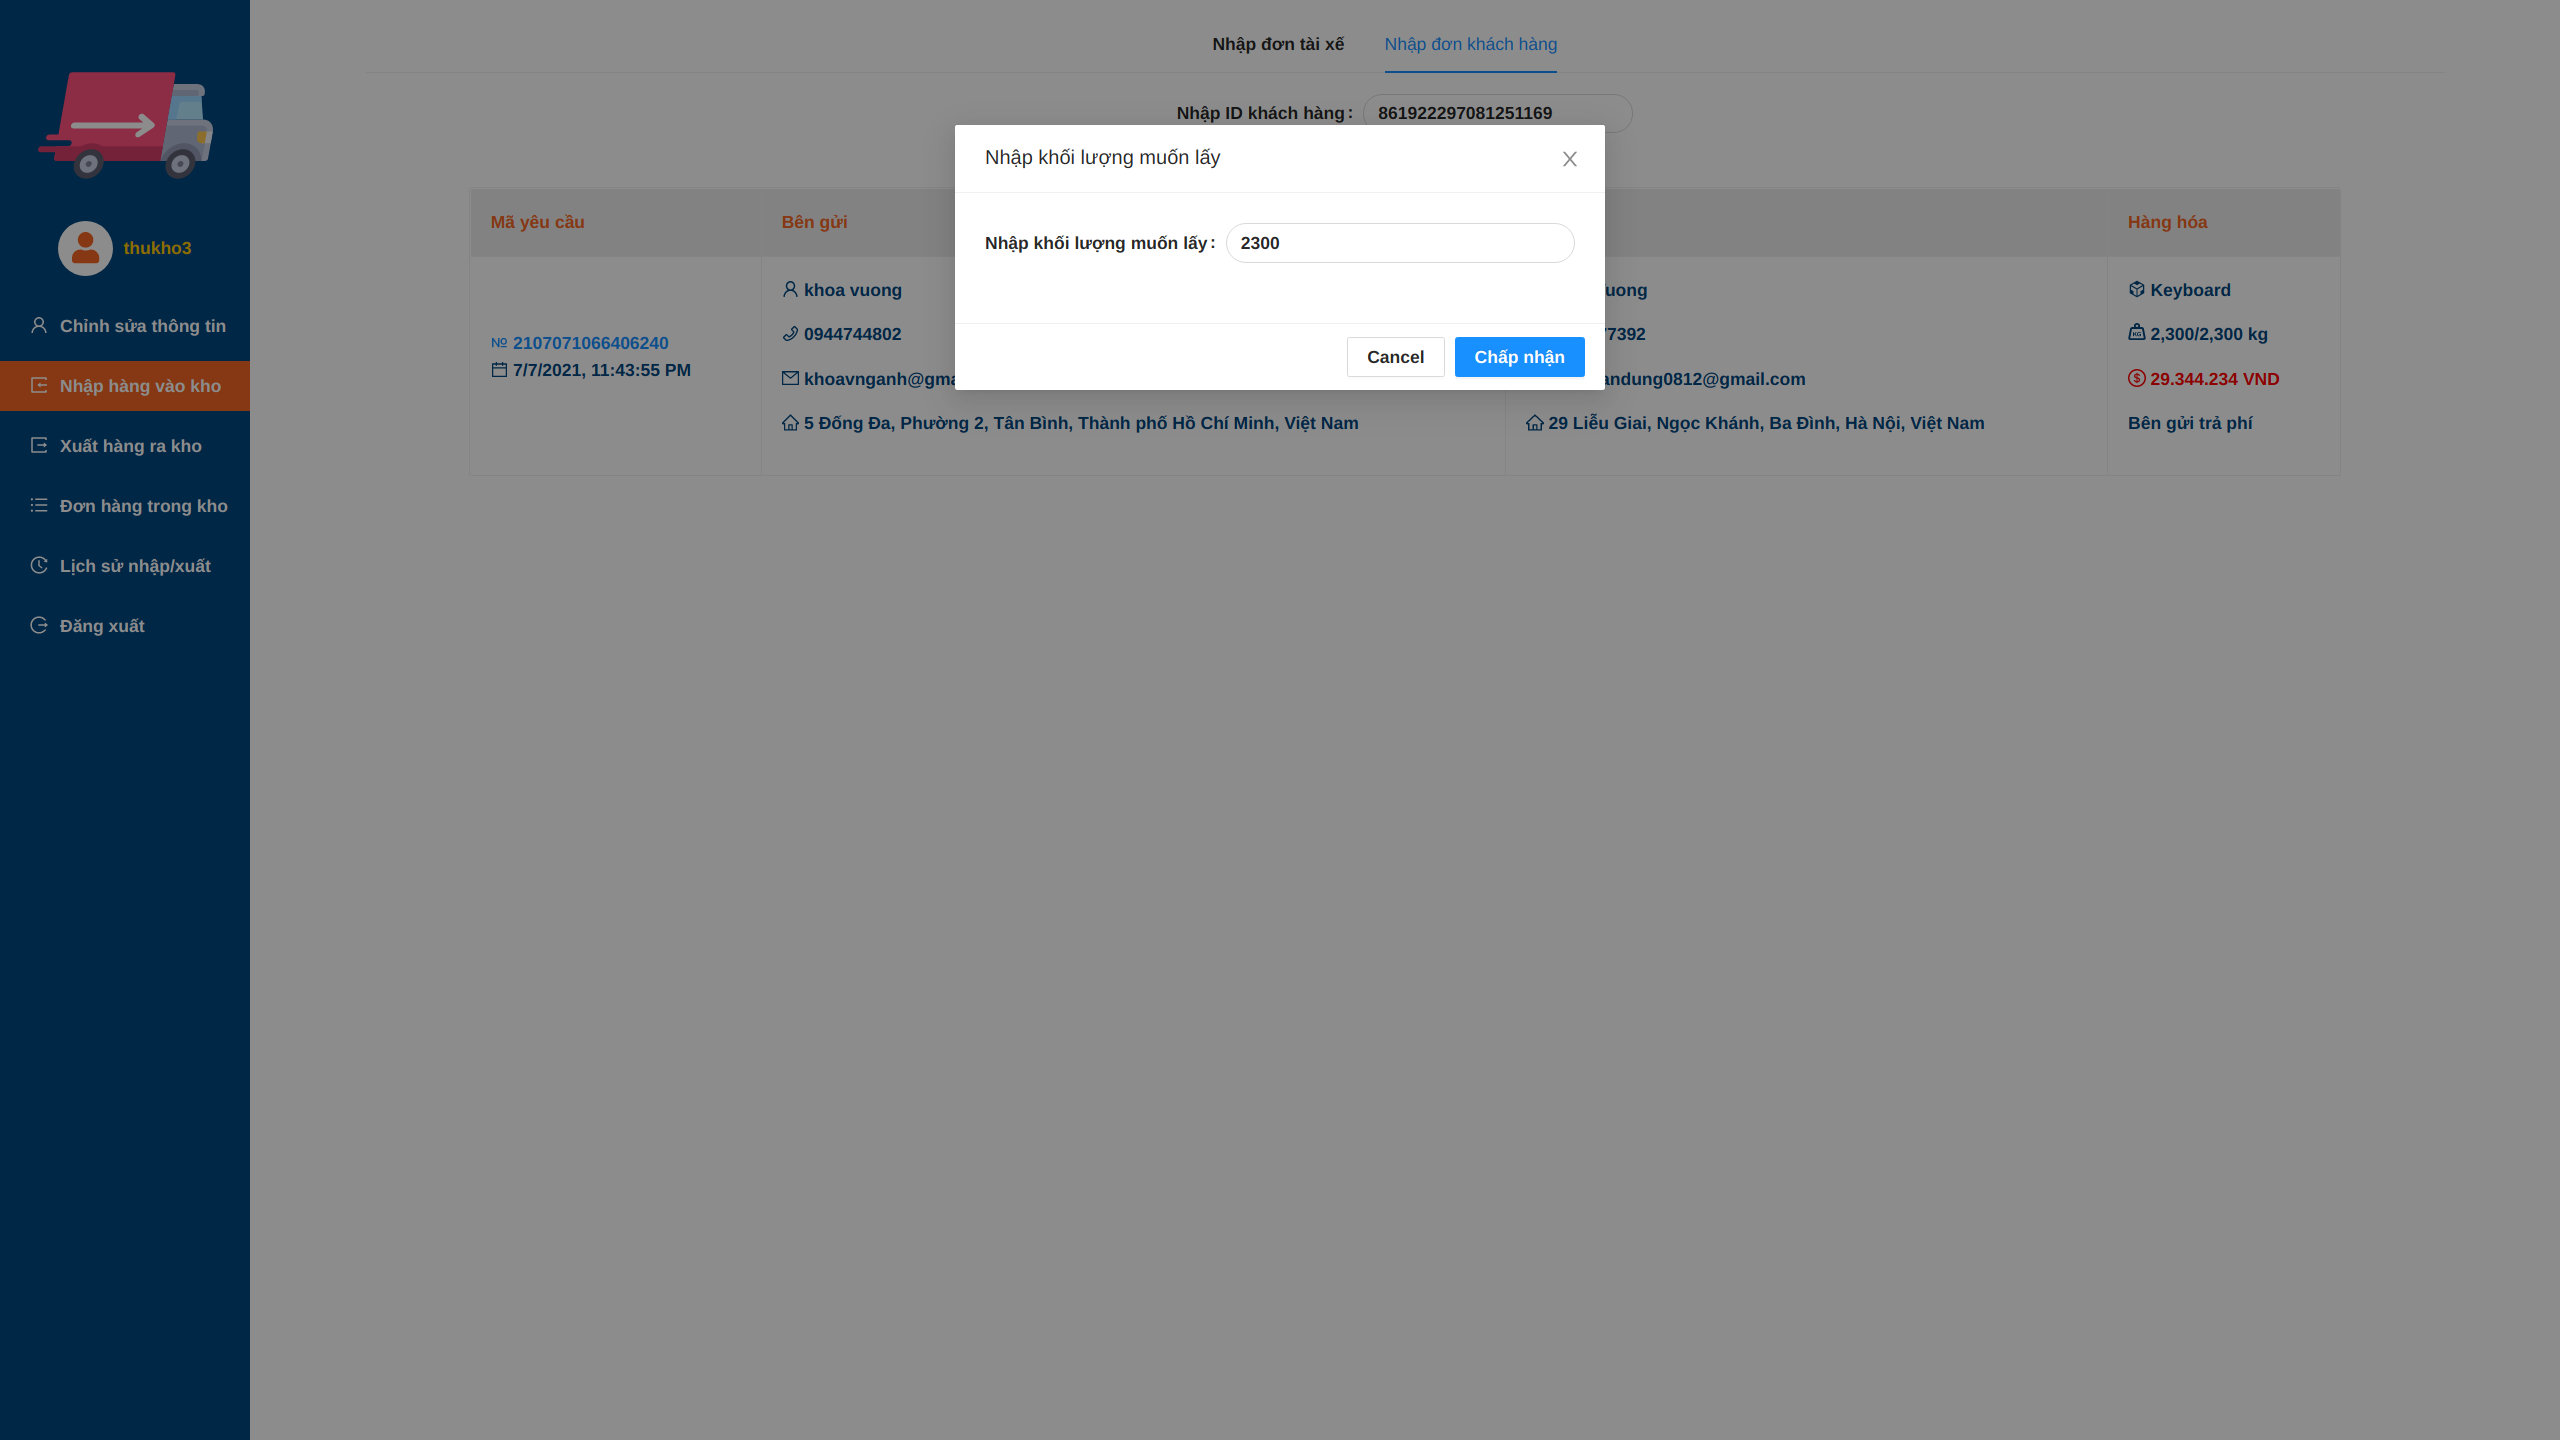
\includegraphics[width=0.8\textwidth]{/stockkeeper/stock_import_customer_detail.png}
					\centering
					\caption{Cho phép nhập khối lượng mà khách muốn nhập vào kho}
				\end{figure}
			
				Chức năng xuất kho có giao diện và tính năng tương tự lúc nhập kho.
				